\documentclass{beamer}

% opacity bugfix: see http://tug.org/pipermail/pdftex/2007-December/007480.html
\pdfpageattr {/Group << /S /Transparency /I true /CS /DeviceRGB>>}

\usepackage[utf8]{inputenc}
\usepackage[OT1]{fontenc}

\usepackage{tikz}
\usetikzlibrary{%
   arrows,%
   calc,%
   fit,%
   patterns,%
   plotmarks,%
   shapes.geometric,%
   shapes.misc,%
   shapes.symbols,%
   shapes.arrows,%
   shapes.callouts,%
   shapes.multipart,%
   shapes.gates.logic.US,%
   shapes.gates.logic.IEC,%
   er,%
   automata,%
   backgrounds,%
   chains,%
   topaths,%
   trees,%
   petri,%
   mindmap,%
   matrix,%
   calendar,%
   folding,%
   fadings,%
   through,%
   patterns,%
   positioning,%
   scopes,%
   decorations.fractals,%
   decorations.shapes,%
   decorations.text,%
   decorations.pathmorphing,%
   decorations.pathreplacing,%
   decorations.footprints,%
   decorations.markings,%
   shadows}
\usepackage{animate}
\usepackage{amssymb, amsmath, amsfonts, enumerate}
%\usepackage{bbold}
\newcommand\hmmax{0}
\usepackage{bm}
%\usepackage{dsfont}
\usepackage{pxfonts}
\usepackage{xcolor}
\usepackage{url}

\usepackage[backend=bibtex,style=authoryear,dashed=false]{biblatex}
\addbibresource{../bib/lundrefs.bib}
%\renewcommand{\bibfont}{\normalfont\scriptsize}
\setlength{\bibhang}{3ex}

\usepackage{hyperref}

\usetheme[official=false,department=none]{tue2008}
%\usefonttheme{default}


%\usetheme[secheader]{Boadilla}
%\setbeamercovered{transparent}
%\setbeamercovered{invisible}
%\setbeamertemplate{navigation symbols}{}
%\setbeamertemplate{bibliography item}[text] % numbered references
%\useoutertheme{infolines}
%\setbeamertemplate{headline}{}
%\setbeamertemplate{footline}{\hspace*{5mm}\hfill\insertframenumber\hspace*{5mm}\vspace{3mm}}
%\setbeamercolor{alerted text}{fg=orange!80!black}

% ------------------------------------------------------------------------------

\newcommand{\vcenterbox}[1]{\ensuremath{\vcenter{\hbox{#1}}}}
%
\newcommand{\reals}{\mathbb{R}}
\newcommand{\posreals}{\reals_{>0}}
\newcommand{\posrealszero}{\reals_{\ge 0}}
\newcommand{\naturals}{\mathbb{N}}

\newcommand{\dd}{\,\mathrm{d}}

\newcommand{\mbf}[1]{\mathbf{#1}}
\newcommand{\bs}[1]{\boldsymbol{#1}}
\renewcommand{\vec}[1]{{\bm#1}}

\newcommand{\uz}{^{(0)}} % upper zero
\newcommand{\un}{^{(n)}} % upper n
\newcommand{\ui}{^{(i)}} % upper i
\newcommand{\uell}{^{(\ell)}} % upper ell

\newcommand{\ul}[1]{\underline{#1}}
\newcommand{\ol}[1]{\overline{#1}}

\newcommand{\Rsys}{R_\text{sys}}
\newcommand{\lRsys}{\ul{R}_\text{sys}}
\newcommand{\uRsys}{\ol{R}_\text{sys}}

\newcommand{\Fsys}{F_\text{sys}}
\newcommand{\lFsys}{\ul{F}_\text{sys}}
\newcommand{\uFsys}{\ol{F}_\text{sys}}

\def\Tsys{T_\text{sys}}

\newcommand{\E}{\operatorname{E}}
\newcommand{\V}{\operatorname{Var}}
\newcommand{\sd}{\operatorname{sd}}

\newcommand{\wei}{\operatorname{Wei}} % Weibull Distribution
\newcommand{\ig}{\operatorname{IG}}   % Inverse Gamma Distribution
\newcommand{\ber}{\operatorname{Bernoulli}} 
\newcommand{\bin}{\operatorname{Binomial}}
\newcommand{\be}{\operatorname{Beta}} 
\newcommand{\bebin}{\operatorname{Beta-binomial}}
\newcommand{\norm}{\operatorname{N}}

\def\then{{\structure{$\rule[0.35ex]{2ex}{0.5ex}\!\!\!\blacktriangleright$}}}
\def\play{{\structure{$\blacktriangleright$}}}
\def\gplus{{\structure{\rule[0.45ex]{1.4ex}{0.4ex}\hspace{-0.9ex}\rule[0.0ex]{0.4ex}{1.3ex}\hspace{0.5ex}}}}
\def\gminus{{\structure{\rule[0.45ex]{1.4ex}{0.4ex}}}}


\def\yz{y\uz}
\def\yn{y\un}
%\def\yi{y\ui}
\newcommand{\yfun}[1]{y^{({#1})}}
\newcommand{\yfunl}[1]{\ul{y}^{({#1})}}
\newcommand{\yfunu}[1]{\ol{y}^{({#1})}}

\def\ykt{y_{k,t}}

\def\ykz{y\uz_k}
\def\ykn{y\un_k}

\def\yktz{y\uz_{k,t}}
\def\yktn{y\un_{k,t}}

\def\yzl{\ul{y}\uz}
\def\yzu{\ol{y}\uz}
\def\ynl{\ul{y}\un}
\def\ynu{\ol{y}\un}
\def\yil{\ul{y}\ui}
\def\yiu{\ol{y}\ui}

\def\ykzl{\ul{y}\uz_k}
\def\ykzu{\ol{y}\uz_k}
\def\yknl{\ul{y}\un_k}
\def\yknu{\ol{y}\un_k}

\def\yktzl{\ul{y}\uz_{k,t}}
\def\yktzu{\ol{y}\uz_{k,t}}
\def\yktnl{\ul{y}\un_{k,t}}
\def\yktnu{\ol{y}\un_{k,t}}


\def\nz{n\uz}
\def\nn{n\un}
%\def\ni{n\ui}
\newcommand{\nfun}[1]{n^{({#1})}}
\newcommand{\nfunl}[1]{\ul{n}^{({#1})}}
\newcommand{\nfunu}[1]{\ol{n}^{({#1})}}

\def\nkz{n\uz_k}
\def\nkn{n\un_k}
\newcommand{\nkzfun}[1]{n\uz_{#1}}

\def\nkt{n_{k,t}}

\def\nktz{n\uz_{k,t}}
\def\nktn{n\un_{k,t}}


\def\nzl{\ul{n}\uz}
\def\nzu{\ol{n}\uz}
\def\nnl{\ul{n}\un}
\def\nnu{\ol{n}\un}
\def\nil{\ul{n}\ui}
\def\niu{\ol{n}\ui}

\def\nkzl{\ul{n}\uz_k}
\def\nkzu{\ol{n}\uz_k}
\def\nknl{\ul{n}\un_k}
\def\nknu{\ol{n}\un_k}

\def\nktzl{\ul{n}\uz_{k,t}}
\def\nktzu{\ol{n}\uz_{k,t}}
\def\nktnl{\ul{n}\un_{k,t}}
\def\nktnu{\ol{n}\un_{k,t}}

\def\taut{\tau(\vec{t})}
\def\taux{\tau(\vec{x})}
\def\ttau{\tilde{\tau}}
\def\ttaut{\ttau(\vec{t})}
\def\ttaux{\ttau(\vec{x})}

\def\MZ{\mathcal{M}\uz}
\def\MN{\mathcal{M}\un}

\def\MkZ{\mathcal{M}\uz_k}
\def\MkN{\mathcal{M}\un_k}

\def\MktZ{\mathcal{M}\uz_{k,t}}
\def\MktN{\mathcal{M}\un_{k,t}}

\def\PZ{\Pi\uz}
\def\PN{\Pi\un}

\def\PkZ{\Pi\uz_k}
\def\PkN{\Pi\un_k}
\newcommand{\PZi}[1]{\Pi\uz_{#1}}

\def\PktZ{\Pi\uz_{k,t}}
\def\PktN{\Pi\un_{k,t}}
\newcommand{\PtZi}[1]{\Pi\uz_{#1,t}}
\newcommand{\PkZi}[1]{\Pi\uz_{k,#1}}

\newcommand{\az}{\alpha\uz}
\newcommand{\an}{\alpha\un}
\newcommand{\bz}{\beta\uz}
\newcommand{\bn}{\beta\un}


\def\blau#1{{\color{tuegreen}#1}}
\def\rot#1{{\color{tuered}#1}}
\def\gruen#1{{\color{tueblue}#1}}

\def\yzr{\rot{\yz}}
\def\ynr{\rot{\yn}}
\def\byzr{\rot{\byz}}
\def\bynr{\rot{\byn}}
\def\yzor{\rot{y\uz_1}}
\def\yzjr{\rot{y\uz_j}}
\def\yzkr{\rot{y\uz_k}}
\def\yzlr{\rot{\yzl}}
\def\yzur{\rot{\yzu}}
\def\ynjr{\rot{y\un_j}}
\def\ynlr{\rot{\ynl}}
\def\ynur{\rot{\ynu}}
\def\yzjlr#1{\rot{\ul{y}\uz_#1}}
\def\yzjur#1{\rot{\ol{y}\uz_#1}}


\def\nzg{\gruen{\nz}}
\def\nng{\gruen{\nn}}
\def\nzlg{\gruen{\nzl}}
\def\nzug{\gruen{\nzu}}
\def\nnlg{\gruen{\nnl}}
\def\nnug{\gruen{\nnu}}

\def\psib{\blau{\psi}}
\def\bpsib{\blau{{b}(\psi)}}


% ------------ shading start
\newsavebox{\tempbox}
\newcommand\leftrightshading[3]{%
  \begin{tikzfadingfrompicture}[name=inputtext]
    \node [text=white] {#1};
  \end{tikzfadingfrompicture}
  \begin{lrbox}{\tempbox}%
    \begin{tikzpicture}
      \node [text=white,inner sep=0pt,outer sep=0pt] (textnode) {#1};
      \shade[path fading=inputtext,fit fading=false,left color=#2,right color=#3]
      (textnode.south west) rectangle (textnode.north east);
    \end{tikzpicture}%
  \end{lrbox}
  % Now we use the fading in another picture:
  \usebox\tempbox{}%
}
% ------------ shading end


%\def\PZc{\mathrm I\!\Pi\uz}
\def\PZc{\leftrightshading{$\mathrm I\!\Pi\uz$}{blue}{red}}
%\def\PNc{\PN}
\def\PNc{\leftrightshading{$\mathrm I\!\Pi\un$}{blue}{red}}



%%\def\blau#1{{\color{lmugreen2}#1}}
%\def\rot#1{{\color{red}#1}}
%\def\gruen#1{{\color{blue}#1}}

\newcommand{\x}{\vec{x}}

\def\tnow{t_\text{now}}
\def\tpnow{t^+_\text{now}}

\newcommand{\comp}[1]{\raisebox{-1mm}{\tikz{\node[%type1
rectangle,rounded corners=0mm,draw,fill=tuepmsgreen!70,thick,inner sep=0pt,minimum size=4mm]{#1};}}}

\newcommand{\cyansec}[1]{\textcolor{tuecyan}{\large\bf #1}}
\newcommand{\cyanalert}[1]{\textcolor{tuecyan}{#1}}
\newcommand{\bluesec}[1]{\textcolor{tueblue}{\large\bf #1}}
\newcommand{\bluealert}[1]{\textcolor{tueblue}{#1}}

\setbeamertemplate{itemize item}{\tiny\raise1.5pt\hbox{\color{tueblue}$\blacktriangleright$}}

% ------------------------------------------------------------------------------


\title{Bayesian Inference and Prior-Data Conflict}

\author{Gero Walter}
\institute{ Eindhoven University of Technology, Eindhoven, NL\\[2ex]
            \url{g.m.walter@tue.nl} \\[2ex]
            
\includegraphics[height=9mm]{logos/tuelogo} \quad
            
\includegraphics[height=9mm]{logos/dinalog-hp} }
\date{2015-12-15}

\begin{document}

\frame{
\titlepage
}

\addtocounter{framenumber}{-1} 

\frame{
\frametitle{Bayesian Inference}
\begin{center}
\begin{tikzpicture} % l b r t
\uncover<1>{\node at (0,0) {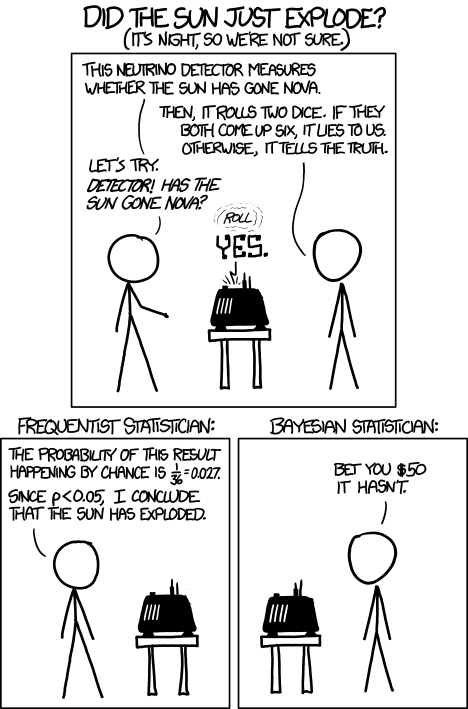
\includegraphics[height=0.9\textheight,trim = 0 300 0 0, clip]{frequentists_vs_bayesians}};}
\uncover<2>{\node at (0,0) {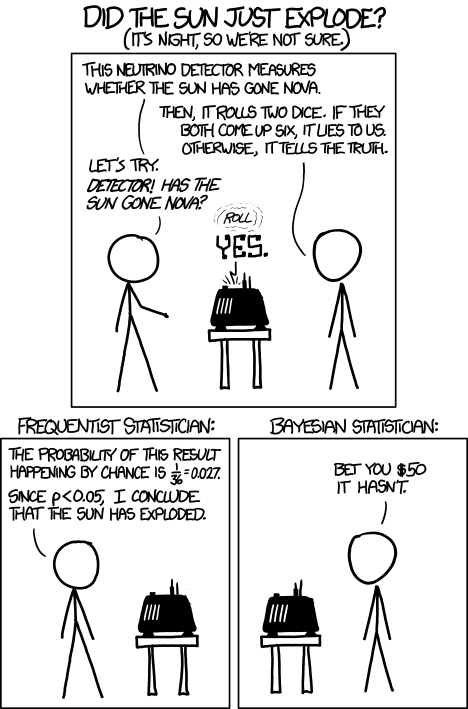
\includegraphics[width=0.9\textwidth,trim = 0 0 0 410, clip]{frequentists_vs_bayesians}};}
\end{tikzpicture}
{\footnotesize \url{https://xkcd.com/1132}}
\end{center}
}


\frame{
\frametitle{Bayesian Inference}
\vspace*{-2ex}
\begin{align*}
\begin{array}{ccccl}
\uncover<1->{\text{expert info}        & + & \text{data}                & \to & \text{complete picture} \\[1.5ex]}
\uncover<2->{\text{prior distribution} & + & \text{sample distribution} & \to & \text{posterior distribution} \\[1.5ex]
 f(\theta) & \times & f(\vec{x} \mid \theta) & \propto & p(\theta \mid \vec{x}) \\
 & & & & \qquad\text{\bluealert{\play\ Bayes' Rule}} \\}
%\uncover<3->{\downarrow & & \downarrow & & \hspace*{3ex} \downarrow \\
\uncover<4->{\text{Beta prior}}   & & \uncover<3->{\text{Binomial}}         & & \uncover<5->{\text{Beta posterior}} \\
\uncover<4->{}                    & & \uncover<3->{\text{distribution}}     & & \uncover<5->{\qquad \text{\bluealert{\play\ conjugacy}}}\\[1ex]
\uncover<4->{p \sim \be(\az,\bz)} & & \uncover<3->{s \mid p \sim \bin(n,p)} & & \uncover<5->{p \mid s \sim \be(\an,\bn)}
\end{array}
\end{align*}
\vspace*{-3ex}
\begin{tikzpicture}
\uncover<6->{%
\node at (0,0) {\parbox{0.99\textwidth}{%
\begin{itemize}
\item conjugate prior makes learning about parameter tractable,\\  %posterior distribution
      just update hyperparameters:\quad $\az \to \an$, $\bz \to \bn$
\item closed form for some inferences: $\E[p\mid s] = \frac{\an}{\an+\bn}$
\end{itemize}}};}
\uncover<3-5>{%
\node at (-0.5,0) {\includegraphics[width=0.25\textwidth]{../course/smallfig-binom}};}
\uncover<4-5>{%
\node at (-4.5,0) {\includegraphics[width=0.25\textwidth]{../course/smallfig-prior}};}
\uncover<5>{%
\node at ( 3.5,0) {\includegraphics[width=0.25\textwidth]{../course/smallfig-posterior}};}
\end{tikzpicture}
}

\frame{
\frametitle{Prior-Data Conflict}
\uncover<1->{What if expert information and data tell different stories?\\[1ex]}
\uncover<2->{%
\begin{block}{Prior-Data Conflict}
\begin{itemize}
\item \emph{informative prior beliefs} and \emph{trusted data}\\ %\rule{0ex}{3ex}\\
(sampling model correct, no outliers, etc.) are in conflict%\\%[2ex]
\item ``[\ldots] the prior [places] its mass primarily on distributions
in the sampling model for which the observed data is surprising''\\
\parencite{2006:evans}
\item there are not enough data to overrule the prior
\end{itemize}
\end{block}}
%\uncover<3->{}
%\uncover<4->{\play\ reparametrization helps to understand effect of prior-data conflict:\\}
}

\frame{\frametitle{Prior-Data Conflict: Example}

%Example Beta-Binom, show point, line, rectangle
\begin{itemize}[<+->]
\item Bernoulli observations: 0/1 observations (failure/success)
\item given: a set of $n$ i.i.d.\ observations and strong prior information
\item we are, e.g., interested in probability for success in next trial
\end{itemize}
\uncover<4->{
\begin{block}{Beta-Binomial Model}
\begin{tabular}{r|lcl}
data :           & $s \mid p$        & $\sim$ & $\bin(n,p)$   \\[0.5ex]
conjugate prior: & $p \mid \az, \bz$ & $\sim$ & $\be(\az,\, \bz)$  \\[0.5ex]
\cline{1-4}
posterior:       & $p \mid \an, \bn$ & $\sim$ & $\be(\an,\, \bn)$\rule{0ex}{2.5ex}
%\quad ($\frac{\tau(\x)}{n} = \frac{s}{n}$)\rule{0ex}{2.5ex}
\end{tabular}
\end{block}
where $s$ = number of successes in the $n$ observed trials}
}

\frame{
\frametitle{Reparametrisation of the Beta Distribution}
\uncover<1->{\play\ reparametrisation helps to understand effect of prior-data conflict:\\}
\begin{tikzpicture}
[pfeil/.style={-latex', line width=1mm, color=tuered, shorten <=1mm},
 cyanrand/.style={rounded corners, text centered, draw=tuecyan!50, inner sep=1mm, line width=0.7mm},
 redbrace/.style={draw=tuered, decoration=brace, decorate, line width=0.8mm},
 redbox/.style={text centered, draw=tuered, inner sep=1.5mm, line width=1mm, minimum width=0.75\textwidth}]
\uncover<1->{%
\node at (0,0.2) {\parbox[c]{\textwidth}{%
\begin{align*}
\nzg &= \az + \bz\,,
&
\yzr &= \frac{\az}{\az + \bz}\,, \quad \text{which are updated as}\\%[1.5ex]
%\\
%\end{align*}
%\intertext{%
%such that
%$\lambda \sim \ig(\nz+1,\nz\yz)$ and $\lambda\mid\mbf{t} \sim \ig(\nell+1,\nell\yell)$,
%where}%
%\begin{align*}
\nng &= \nzg + n\,, 
&
\ynr &=  \frac{\nzg}{\nzg + n} \, \yzr + \frac{n}{\nzg + n} \cdot \frac{s}{n}
\end{align*}
}};}
\uncover<2->{%
\node[cyanrand] (yz) at (-0.9,-1.9) {$\yzr = \E[p]$};
\draw [pfeil] (yz.north east) to [out= 30,in=260] ( 0.9,-0.65);
\draw [pfeil] (yz.north west) to [out=130,in=240] (-1.7,0.4);}
\uncover<3->{%
\node[cyanrand] (yn) at ( 1.4,-1.9) {$\ynr = \E[p \mid s]$};
\draw [pfeil] (yn.north)      to [out=130,in=280] (-1.4,-0.65);}
\uncover<4->{%
\node[cyanrand] (ml) at ( 4.3,-1.9) {ML estimator $\hat{p}$};
\draw [pfeil] (ml.north)      to [out=100,in=330] (3.6,-0.65);}
\uncover<5->{%
\node[cyanrand] (nz) at (-4  ,-1.9) {$\nzg =$ pseudocounts};
\draw [pfeil] (nz.north)      to [out=90,in=270] (-4.0,-0.65);
\draw [pfeil] (nz.north west) to [out=95,in=240] (-5.2, 0.5);}
\uncover<6->{%
\node[redbox] at (0,-2.8) {$\E[p \mid s] = \ynr$ is a weighted average of $\E[p]$ and $\hat{p}$!};}
\uncover<7->{%
\node[redbox] at (0,-4.0) {$\V[p \mid s] = \dfrac{\ynr (1-\ynr)}{\nng + 1}$ decreases with $n$!};}
\end{tikzpicture}
}

\frame{\frametitle{Beta-Binomial Model (BBM)}

\hspace*{-12ex}
\begin{columns}%[T]
\begin{column}{0.55\textwidth}
\begin{tikzpicture}
\pgftransformscale{0.025}
\uncover<1>{
% Created by tikzDevice version 0.5.0 on 2011-07-18 16:47:19
\begin{scope}
\path[clip] ( 55.20, 49.20) rectangle (250.54,221.74);
\definecolor[named]{drawColor}{rgb}{0.82,0.27,0.19}
\definecolor[named]{fillColor}{rgb}{0.88,0.08,0.52}
\definecolor[named]{drawColor}{rgb}{0.00,0.00,0.00}
\definecolor[named]{fillColor}{rgb}{0.00,0.00,0.00}

\draw[color=drawColor,line cap=round,line join=round,fill=fillColor,] ( 96.89,175.41) circle (  2.25);
\end{scope}
\begin{scope}
\path[clip] (  0.00,  0.00) rectangle (252.94,252.94);
\definecolor[named]{drawColor}{rgb}{0.82,0.27,0.19}
\definecolor[named]{fillColor}{rgb}{0.88,0.08,0.52}
\definecolor[named]{drawColor}{rgb}{0.00,0.00,0.00}

\draw[color=drawColor,line cap=round,line join=round,fill opacity=0.00,] ( 71.05, 49.20) -- (243.31, 49.20);

\draw[color=drawColor,line cap=round,line join=round,fill opacity=0.00,] ( 71.05, 49.20) -- ( 71.05, 43.20);

\draw[color=drawColor,line cap=round,line join=round,fill opacity=0.00,] (114.11, 49.20) -- (114.11, 43.20);

\draw[color=drawColor,line cap=round,line join=round,fill opacity=0.00,] (157.18, 49.20) -- (157.18, 43.20);

\draw[color=drawColor,line cap=round,line join=round,fill opacity=0.00,] (200.24, 49.20) -- (200.24, 43.20);

\draw[color=drawColor,line cap=round,line join=round,fill opacity=0.00,] (243.31, 49.20) -- (243.31, 43.20);

\node[color=drawColor,anchor=base,inner sep=0pt, outer sep=0pt, scale=  0.90] at ( 71.05, 25.20) {5%
};

\node[color=drawColor,anchor=base,inner sep=0pt, outer sep=0pt, scale=  0.90] at (114.11, 25.20) {10%
};

\node[color=drawColor,anchor=base,inner sep=0pt, outer sep=0pt, scale=  0.90] at (157.18, 25.20) {15%
};

\node[color=drawColor,anchor=base,inner sep=0pt, outer sep=0pt, scale=  0.90] at (200.24, 25.20) {20%
};

\node[color=drawColor,anchor=base,inner sep=0pt, outer sep=0pt, scale=  0.90] at (243.31, 25.20) {25%
};

\draw[color=drawColor,line cap=round,line join=round,fill opacity=0.00,] ( 55.20, 55.59) -- ( 55.20,215.35);

\draw[color=drawColor,line cap=round,line join=round,fill opacity=0.00,] ( 55.20, 55.59) -- ( 49.20, 55.59);

\draw[color=drawColor,line cap=round,line join=round,fill opacity=0.00,] ( 55.20, 87.54) -- ( 49.20, 87.54);

\draw[color=drawColor,line cap=round,line join=round,fill opacity=0.00,] ( 55.20,119.50) -- ( 49.20,119.50);

\draw[color=drawColor,line cap=round,line join=round,fill opacity=0.00,] ( 55.20,151.45) -- ( 49.20,151.45);

\draw[color=drawColor,line cap=round,line join=round,fill opacity=0.00,] ( 55.20,183.40) -- ( 49.20,183.40);

\draw[color=drawColor,line cap=round,line join=round,fill opacity=0.00,] ( 55.20,215.35) -- ( 49.20,215.35);

\node[rotate= 90.00,color=drawColor,anchor=base,inner sep=0pt, outer sep=0pt, scale=  0.90] at ( 43.20, 55.59) {0.0%
};

\node[rotate= 90.00,color=drawColor,anchor=base,inner sep=0pt, outer sep=0pt, scale=  0.90] at ( 43.20, 87.54) {0.2%
};

\node[rotate= 90.00,color=drawColor,anchor=base,inner sep=0pt, outer sep=0pt, scale=  0.90] at ( 43.20,119.50) {0.4%
};

\node[rotate= 90.00,color=drawColor,anchor=base,inner sep=0pt, outer sep=0pt, scale=  0.90] at ( 43.20,151.45) {0.6%
};

\node[rotate= 90.00,color=drawColor,anchor=base,inner sep=0pt, outer sep=0pt, scale=  0.90] at ( 43.20,183.40) {0.8%
};

\node[rotate= 90.00,color=drawColor,anchor=base,inner sep=0pt, outer sep=0pt, scale=  0.90] at ( 43.20,215.35) {1.0%
};

\draw[color=drawColor,line cap=round,line join=round,fill opacity=0.00,] ( 55.20, 49.20) --
    (250.54, 49.20) --
    (250.54,221.74) --
    ( 55.20,221.74) --
    ( 55.20, 49.20);
\end{scope}
\begin{scope}
\path[clip] (  0.00,  0.00) rectangle (252.94,252.94);
\definecolor[named]{drawColor}{rgb}{0.82,0.27,0.19}
\definecolor[named]{fillColor}{rgb}{0.88,0.08,0.52}
\definecolor[named]{drawColor}{rgb}{0.00,0.00,0.00}

\node[color=drawColor,anchor=base,inner sep=0pt, outer sep=0pt, scale=  1.00] at (152.87,  1.20) {$\gruen{\nz}$ resp. $\gruen{\nn}$%
};

\node[rotate= 90.00,color=drawColor,anchor=base,inner sep=0pt, outer sep=0pt, scale=  1.00] at ( 19.20,135.47) {$\rot{\yz}$ resp. $\rot{\yn}$%
};
\end{scope}

}
\uncover<2>{
% Created by tikzDevice version 0.5.0 on 2011-07-18 12:18:44
\begin{scope}
\path[clip] ( 55.20, 49.20) rectangle (250.54,221.74);
\definecolor[named]{fillColor}{rgb}{0.88,0.08,0.52}
\definecolor[named]{drawColor}{rgb}{0.00,0.00,0.00}
\definecolor[named]{fillColor}{rgb}{0.00,0.00,0.00}

\draw[color=drawColor,line cap=round,line join=round,fill=fillColor,] ( 96.89,175.41) circle (  2.25);

\draw[color=drawColor,line cap=round,line join=round,fill=fillColor,] (234.70,175.41) circle (  2.25);
\end{scope}
\begin{scope}
\path[clip] (  0.00,  0.00) rectangle (252.94,252.94);
\definecolor[named]{fillColor}{rgb}{0.88,0.08,0.52}
\definecolor[named]{drawColor}{rgb}{0.00,0.00,0.00}

\draw[color=drawColor,line cap=round,line join=round,fill opacity=0.00,] ( 71.05, 49.20) -- (243.31, 49.20);

\draw[color=drawColor,line cap=round,line join=round,fill opacity=0.00,] ( 71.05, 49.20) -- ( 71.05, 43.20);

\draw[color=drawColor,line cap=round,line join=round,fill opacity=0.00,] (114.11, 49.20) -- (114.11, 43.20);

\draw[color=drawColor,line cap=round,line join=round,fill opacity=0.00,] (157.18, 49.20) -- (157.18, 43.20);

\draw[color=drawColor,line cap=round,line join=round,fill opacity=0.00,] (200.24, 49.20) -- (200.24, 43.20);

\draw[color=drawColor,line cap=round,line join=round,fill opacity=0.00,] (243.31, 49.20) -- (243.31, 43.20);

\node[color=drawColor,anchor=base,inner sep=0pt, outer sep=0pt, scale=  0.90] at ( 71.05, 25.20) {5%
};

\node[color=drawColor,anchor=base,inner sep=0pt, outer sep=0pt, scale=  0.90] at (114.11, 25.20) {10%
};

\node[color=drawColor,anchor=base,inner sep=0pt, outer sep=0pt, scale=  0.90] at (157.18, 25.20) {15%
};

\node[color=drawColor,anchor=base,inner sep=0pt, outer sep=0pt, scale=  0.90] at (200.24, 25.20) {20%
};

\node[color=drawColor,anchor=base,inner sep=0pt, outer sep=0pt, scale=  0.90] at (243.31, 25.20) {25%
};

\draw[color=drawColor,line cap=round,line join=round,fill opacity=0.00,] ( 55.20, 55.59) -- ( 55.20,215.35);

\draw[color=drawColor,line cap=round,line join=round,fill opacity=0.00,] ( 55.20, 55.59) -- ( 49.20, 55.59);

\draw[color=drawColor,line cap=round,line join=round,fill opacity=0.00,] ( 55.20, 87.54) -- ( 49.20, 87.54);

\draw[color=drawColor,line cap=round,line join=round,fill opacity=0.00,] ( 55.20,119.50) -- ( 49.20,119.50);

\draw[color=drawColor,line cap=round,line join=round,fill opacity=0.00,] ( 55.20,151.45) -- ( 49.20,151.45);

\draw[color=drawColor,line cap=round,line join=round,fill opacity=0.00,] ( 55.20,183.40) -- ( 49.20,183.40);

\draw[color=drawColor,line cap=round,line join=round,fill opacity=0.00,] ( 55.20,215.35) -- ( 49.20,215.35);

\node[rotate= 90.00,color=drawColor,anchor=base,inner sep=0pt, outer sep=0pt, scale=  0.90] at ( 43.20, 55.59) {0.0%
};

\node[rotate= 90.00,color=drawColor,anchor=base,inner sep=0pt, outer sep=0pt, scale=  0.90] at ( 43.20, 87.54) {0.2%
};

\node[rotate= 90.00,color=drawColor,anchor=base,inner sep=0pt, outer sep=0pt, scale=  0.90] at ( 43.20,119.50) {0.4%
};

\node[rotate= 90.00,color=drawColor,anchor=base,inner sep=0pt, outer sep=0pt, scale=  0.90] at ( 43.20,151.45) {0.6%
};

\node[rotate= 90.00,color=drawColor,anchor=base,inner sep=0pt, outer sep=0pt, scale=  0.90] at ( 43.20,183.40) {0.8%
};

\node[rotate= 90.00,color=drawColor,anchor=base,inner sep=0pt, outer sep=0pt, scale=  0.90] at ( 43.20,215.35) {1.0%
};

\draw[color=drawColor,line cap=round,line join=round,fill opacity=0.00,] ( 55.20, 49.20) --
    (250.54, 49.20) --
    (250.54,221.74) --
    ( 55.20,221.74) --
    ( 55.20, 49.20);
\end{scope}
\begin{scope}
\path[clip] (  0.00,  0.00) rectangle (252.94,252.94);
\definecolor[named]{fillColor}{rgb}{0.88,0.08,0.52}
\definecolor[named]{drawColor}{rgb}{0.00,0.00,0.00}

\node[color=drawColor,anchor=base,inner sep=0pt, outer sep=0pt, scale=  1.00] at (152.87,  1.20) {$\gruen{\nz}$ resp. $\gruen{\nn}$%
};

\node[rotate= 90.00,color=drawColor,anchor=base,inner sep=0pt, outer sep=0pt, scale=  1.00] at ( 19.20,135.47) {$\rot{\yz}$ resp. $\rot{\yn}$%
};
\end{scope}

\draw[-stealth,very thick] (110,175) -- (220,175) node [above,midway] {12 out of 16};
}
\uncover<3->{
% Created by tikzDevice version 0.5.0 on 2011-07-18 12:18:48
\begin{scope}
\path[clip] ( 55.20, 49.20) rectangle (250.54,221.74);
\definecolor[named]{drawColor}{rgb}{0.60,0.27,0.19}
\definecolor[named]{fillColor}{rgb}{0.88,0.08,0.52}
\definecolor[named]{drawColor}{rgb}{0.00,0.00,0.00}
\definecolor[named]{fillColor}{rgb}{0.00,0.00,0.00}

\draw[color=drawColor,line cap=round,line join=round,fill=fillColor,] ( 96.89, 95.53) circle (  2.25);

\draw[color=drawColor,line cap=round,line join=round,fill=fillColor,] ( 96.89,175.41) circle (  2.25);

\draw[color=drawColor,line cap=round,line join=round,fill=fillColor,] (234.70,175.41) circle (  2.25);
\end{scope}
\begin{scope}
\path[clip] (  0.00,  0.00) rectangle (252.94,252.94);
\definecolor[named]{drawColor}{rgb}{0.60,0.27,0.19}
\definecolor[named]{fillColor}{rgb}{0.88,0.08,0.52}
\definecolor[named]{drawColor}{rgb}{0.00,0.00,0.00}

\draw[color=drawColor,line cap=round,line join=round,fill opacity=0.00,] ( 71.05, 49.20) -- (243.31, 49.20);

\draw[color=drawColor,line cap=round,line join=round,fill opacity=0.00,] ( 71.05, 49.20) -- ( 71.05, 43.20);

\draw[color=drawColor,line cap=round,line join=round,fill opacity=0.00,] (114.11, 49.20) -- (114.11, 43.20);

\draw[color=drawColor,line cap=round,line join=round,fill opacity=0.00,] (157.18, 49.20) -- (157.18, 43.20);

\draw[color=drawColor,line cap=round,line join=round,fill opacity=0.00,] (200.24, 49.20) -- (200.24, 43.20);

\draw[color=drawColor,line cap=round,line join=round,fill opacity=0.00,] (243.31, 49.20) -- (243.31, 43.20);

\node[color=drawColor,anchor=base,inner sep=0pt, outer sep=0pt, scale=  0.90] at ( 71.05, 25.20) {5%
};

\node[color=drawColor,anchor=base,inner sep=0pt, outer sep=0pt, scale=  0.90] at (114.11, 25.20) {10%
};

\node[color=drawColor,anchor=base,inner sep=0pt, outer sep=0pt, scale=  0.90] at (157.18, 25.20) {15%
};

\node[color=drawColor,anchor=base,inner sep=0pt, outer sep=0pt, scale=  0.90] at (200.24, 25.20) {20%
};

\node[color=drawColor,anchor=base,inner sep=0pt, outer sep=0pt, scale=  0.90] at (243.31, 25.20) {25%
};

\draw[color=drawColor,line cap=round,line join=round,fill opacity=0.00,] ( 55.20, 55.59) -- ( 55.20,215.35);

\draw[color=drawColor,line cap=round,line join=round,fill opacity=0.00,] ( 55.20, 55.59) -- ( 49.20, 55.59);

\draw[color=drawColor,line cap=round,line join=round,fill opacity=0.00,] ( 55.20, 87.54) -- ( 49.20, 87.54);

\draw[color=drawColor,line cap=round,line join=round,fill opacity=0.00,] ( 55.20,119.50) -- ( 49.20,119.50);

\draw[color=drawColor,line cap=round,line join=round,fill opacity=0.00,] ( 55.20,151.45) -- ( 49.20,151.45);

\draw[color=drawColor,line cap=round,line join=round,fill opacity=0.00,] ( 55.20,183.40) -- ( 49.20,183.40);

\draw[color=drawColor,line cap=round,line join=round,fill opacity=0.00,] ( 55.20,215.35) -- ( 49.20,215.35);

\node[rotate= 90.00,color=drawColor,anchor=base,inner sep=0pt, outer sep=0pt, scale=  0.90] at ( 43.20, 55.59) {0.0%
};

\node[rotate= 90.00,color=drawColor,anchor=base,inner sep=0pt, outer sep=0pt, scale=  0.90] at ( 43.20, 87.54) {0.2%
};

\node[rotate= 90.00,color=drawColor,anchor=base,inner sep=0pt, outer sep=0pt, scale=  0.90] at ( 43.20,119.50) {0.4%
};

\node[rotate= 90.00,color=drawColor,anchor=base,inner sep=0pt, outer sep=0pt, scale=  0.90] at ( 43.20,151.45) {0.6%
};

\node[rotate= 90.00,color=drawColor,anchor=base,inner sep=0pt, outer sep=0pt, scale=  0.90] at ( 43.20,183.40) {0.8%
};

\node[rotate= 90.00,color=drawColor,anchor=base,inner sep=0pt, outer sep=0pt, scale=  0.90] at ( 43.20,215.35) {1.0%
};

\draw[color=drawColor,line cap=round,line join=round,fill opacity=0.00,] ( 55.20, 49.20) --
    (250.54, 49.20) --
    (250.54,221.74) --
    ( 55.20,221.74) --
    ( 55.20, 49.20);
\end{scope}
\begin{scope}
\path[clip] (  0.00,  0.00) rectangle (252.94,252.94);
\definecolor[named]{drawColor}{rgb}{0.60,0.27,0.19}
\definecolor[named]{fillColor}{rgb}{0.88,0.08,0.52}
\definecolor[named]{drawColor}{rgb}{0.00,0.00,0.00}

\node[color=drawColor,anchor=base,inner sep=0pt, outer sep=0pt, scale=  1.00] at (152.87,  1.20) {$\gruen{\nz}$ resp. $\gruen{\nn}$%
};

\node[rotate= 90.00,color=drawColor,anchor=base,inner sep=0pt, outer sep=0pt, scale=  1.00] at ( 19.20,135.47) {$\rot{\yz}$ resp. $\rot{\yn}$%
};
\end{scope}

\draw[-stealth,very thick,gray] (110,175) -- (220,175) node [above,midway,gray] {12 out of 16};
}
\uncover<4->{
\draw[-stealth,very thick] (110,102) -- (220,167) node [above,midway,sloped] {16 out of 16};
}
\end{tikzpicture}
\end{column}
\begin{column}{0.45\textwidth}
\uncover<1->{%
\begin{block}{no conflict:}
prior $\nzg = 8$, $\yzr = 0.75$\\
data $s/n = 12/16 = 0.75$
\end{block}
} %
\uncover<2->{%
\vspace*{-1.5ex}\centerline{\color{tueblue} $\blacktriangledown$}\vspace*{-1.5ex}
\begin{block}{}
$\nng = 24$, $\ynr = 0.75$
\end{block}
} %
\uncover<4->{%
\vspace*{-1.5ex}\centerline{\color{tueblue} $\blacktriangle$}\vspace*{-1.5ex}
}
\uncover<3->{%
\begin{block}{prior-data conflict:}
prior $\nzg = 8$, $\yzr = 0.25$\\
data $s/n = 16/16 = 1$
\end{block}
} %
\uncover<0>{%
\vspace*{-1.5ex}\centerline{\color{tueblue} $\blacktriangledown$}\vspace*{-1.5ex}
\begin{block}{}
$\nng \in [20, 24]$, $\ynr \in [0.73, 0.86]$
\end{block}
} %
%\uncover<5->{ %
%\then\ same predictive prob.\ P!
%}
\end{column}
\end{columns}
}

\frame{\frametitle{Canonical Conjugate Priors}

\uncover<1->{%
Averaging property holds \alert{\emph{for all conjugate models}} (!)
\begin{block}%
{$(x_1, \ldots, x_n) = \x \stackrel{iid}{\sim}$ canonical exponential family} %(Bernardo and Smith, 1994)
%, i.e.
%\begin{align*}
\centering
$f(\x \mid \theta) \propto \exp\big\{\langle \psib, \tau(\x) \rangle - n \bpsib \big\}
\qquad \Big[ \psib \text{ transformation of } \theta \Big]$\\[1.5ex]
%\end{align*}
(includes Binomial, Multinomial, Normal, Poisson, Exponential, \ldots )%\\[2ex]
\end{block}}
\vspace*{-3ex}%
\begin{align*}
\uncover<2->{%
&\text{\play\ conjugate prior:} &
f(\psib\mid\nzg,\yzr) \hspace*{2ex}
&\propto \exp\big\{ \nzg \big[\langle \psib, \yzr \rangle - \bpsib\big]\big\} \\}
\uncover<3->{%
&\text{\play\ (conjugate) posterior:} &
f(\psib\mid\nzg,\yzr,\vec{x})
%p(\psib\mid\nng,\ynr) \hspace*{2ex}
&\propto \exp\big\{ \nng \big[\langle \psib, \ynr \rangle - \bpsib\big]\big\} }%\quad \mbox{where}
\end{align*}
\vspace*{-4ex}%
\uncover<3->{%
\begin{align*}
\mbox{where}\quad \ynr &= \frac{\nzg}{\nzg + n} \cdot \yzr + \frac{n}{\nzg + n} \cdot \frac{\tau(\x)}{n} & &\mbox{and} & \nng &= \nzg + n
\end{align*}}
\vspace*{-2ex}%
\uncover<4->{%
\begin{itemize}
\item $\nzg$ determines \alert{spread} and \alert{learning speed}
\item $\yzr$ = \alert{prior expectation} of $\tau(\x)/n$}
\end{itemize}
}

\frame{
\frametitle{Imprecise / Interval Probability}
\begin{itemize}[<+->]
\item Averaging property holds \alert{\emph{for all conjugate models}} (!)\\
\cyanalert{Can we mitigate this and still keep tractability?}
\item Prior $f(p)$ is a collection of probability statements:
\begin{center}
$\int_a^b f(p) \dd p = P(a \le p \le b)$\\[1.5ex]
%Reliability function $R(t)$ is a collection of probability statements:\\
%$R(t) =$ probability that the system survives past $t$.\\
%%In the long run, what percentage of components survive past $t$?\\
\cyanalert{How can we express uncertainty\\ about these probability statements?}
\end{center}
\item[\play] \textbf{Add \alert{imprecision} as new modelling dimension:\\
\alert{Sets of priors} model uncertainty in probability statements\\
and allow to better model partial or vague information on $p$.}
\item Separate uncertainty \emph{within the model} (probability statements)\\
from uncertainty \emph{about the model} (how certain about statements) %(which parameters).
\item Can also be seen as systematic sensitivity analysis\\
or robust Bayesian approach.
\end{itemize}
}

\frame{
\frametitle{Sets of Prior Distributions}
\uncover<1->{%
\begin{block}{Uncertainty about probability statements}
\centerline{smaller sets $=$ more precise probability statements}
\vspace*{1ex}
\parbox[t]{0.45\textwidth}{\centering \textbf{Lottery A}\\
                          Number of winning tickets:\\
                          exactly known as 5 out of 100\\
                          \play\ $P(\text{win}) = 5/100$}
\qquad
\parbox[t]{0.45\textwidth}{\centering \textbf{Lottery B}\\
                          Number of winning tickets:\\
                          not exactly known, supposedly\\
                          between 1 and 7 out of 100\\
                          \play\ $P(\text{win}) = [1/100,\, 7/100]$}
\end{block}}
\uncover<2->{%
Let hyperparameters $(\nzg, \yzr)$ vary in a set $\PZc$ \play\ set of priors $\MZ$\\[1ex]}
\uncover<3->{%
Sets of priors $\to$ sets of posteriors by updating element by element:\\
GBR \parencite{1991:walley} ensures \emph{coherence} {\small (a consistency property)}\\[1ex]}
\uncover<4->{%
Set of posteriors $\MN$ via $\PNc = \big\{(\nng,\ynr) \colon (\nzg,\yzr) \in \PZc \big\}$\\
Bounds for inferences (point estimate, \ldots) by min/max over $\PZc$.
%\textcite{2009:WalterAugustin}, \textcite{2013:diss-gw}: $\PZc = [\nzlg, \nzug] \times [\yzlr, \yzur]$\\
%gives tractability \& meaningful reaction to prior-data conflict:
%\begin{itemize}
%\item larger set of posteriors %$\to$ larger intervals
%\item more imprecise / cautious probability statements
%\end{itemize}
}
}

\frame{\frametitle{Imprecise BBM with $\nz$ fixed}
%IDM (Walley 1996)\\ Quaghebeur \& de Cooman (2005)
IDM \parencite{1996:walley::idm}; \textcite{2005:quaeghebeurcooman}
\hspace*{-12ex}
\begin{columns}%[T]
\begin{column}{0.55\textwidth}
\begin{tikzpicture}
\pgftransformscale{0.025}
\uncover<1>{
% Created by tikzDevice version 0.5.0 on 2011-07-19 12:27:34
\begin{scope}
\path[clip] ( 55.20, 49.20) rectangle (250.54,221.74);
\definecolor[named]{drawColor}{rgb}{0.38,0.64,0.19}
\definecolor[named]{fillColor}{rgb}{0.88,0.08,0.52}
\definecolor[named]{drawColor}{rgb}{0.75,0.75,0.75}
\definecolor[named]{fillColor}{rgb}{0.75,0.75,0.75}

\draw[color=drawColor,line cap=rect,line join=round,fill=fillColor,] ( 96.89, 95.53) circle (  2.25);

\draw[color=drawColor,line cap=rect,line join=round,fill=fillColor,] ( 96.89,175.41) circle (  2.25);

\draw[color=drawColor,line cap=rect,line join=round,fill=fillColor,] (234.70,175.41) circle (  2.25);
\end{scope}
\begin{scope}
\path[clip] (  0.00,  0.00) rectangle (252.94,252.94);
\definecolor[named]{drawColor}{rgb}{0.38,0.64,0.19}
\definecolor[named]{fillColor}{rgb}{0.88,0.08,0.52}
\definecolor[named]{drawColor}{rgb}{0.00,0.00,0.00}

\draw[color=drawColor,line cap=rect,line join=round,fill opacity=0.00,] ( 71.05, 49.20) -- (243.31, 49.20);

\draw[color=drawColor,line cap=rect,line join=round,fill opacity=0.00,] ( 71.05, 49.20) -- ( 71.05, 43.20);

\draw[color=drawColor,line cap=rect,line join=round,fill opacity=0.00,] (114.11, 49.20) -- (114.11, 43.20);

\draw[color=drawColor,line cap=rect,line join=round,fill opacity=0.00,] (157.18, 49.20) -- (157.18, 43.20);

\draw[color=drawColor,line cap=rect,line join=round,fill opacity=0.00,] (200.24, 49.20) -- (200.24, 43.20);

\draw[color=drawColor,line cap=rect,line join=round,fill opacity=0.00,] (243.31, 49.20) -- (243.31, 43.20);

\node[color=drawColor,anchor=base,inner sep=0pt, outer sep=0pt, scale=  0.90] at ( 71.05, 25.20) {5%
};

\node[color=drawColor,anchor=base,inner sep=0pt, outer sep=0pt, scale=  0.90] at (114.11, 25.20) {10%
};

\node[color=drawColor,anchor=base,inner sep=0pt, outer sep=0pt, scale=  0.90] at (157.18, 25.20) {15%
};

\node[color=drawColor,anchor=base,inner sep=0pt, outer sep=0pt, scale=  0.90] at (200.24, 25.20) {20%
};

\node[color=drawColor,anchor=base,inner sep=0pt, outer sep=0pt, scale=  0.90] at (243.31, 25.20) {25%
};

\draw[color=drawColor,line cap=rect,line join=round,fill opacity=0.00,] ( 55.20, 55.59) -- ( 55.20,215.35);

\draw[color=drawColor,line cap=rect,line join=round,fill opacity=0.00,] ( 55.20, 55.59) -- ( 49.20, 55.59);

\draw[color=drawColor,line cap=rect,line join=round,fill opacity=0.00,] ( 55.20, 87.54) -- ( 49.20, 87.54);

\draw[color=drawColor,line cap=rect,line join=round,fill opacity=0.00,] ( 55.20,119.50) -- ( 49.20,119.50);

\draw[color=drawColor,line cap=rect,line join=round,fill opacity=0.00,] ( 55.20,151.45) -- ( 49.20,151.45);

\draw[color=drawColor,line cap=rect,line join=round,fill opacity=0.00,] ( 55.20,183.40) -- ( 49.20,183.40);

\draw[color=drawColor,line cap=rect,line join=round,fill opacity=0.00,] ( 55.20,215.35) -- ( 49.20,215.35);

\node[rotate= 90.00,color=drawColor,anchor=base,inner sep=0pt, outer sep=0pt, scale=  0.90] at ( 43.20, 55.59) {0.0%
};

\node[rotate= 90.00,color=drawColor,anchor=base,inner sep=0pt, outer sep=0pt, scale=  0.90] at ( 43.20, 87.54) {0.2%
};

\node[rotate= 90.00,color=drawColor,anchor=base,inner sep=0pt, outer sep=0pt, scale=  0.90] at ( 43.20,119.50) {0.4%
};

\node[rotate= 90.00,color=drawColor,anchor=base,inner sep=0pt, outer sep=0pt, scale=  0.90] at ( 43.20,151.45) {0.6%
};

\node[rotate= 90.00,color=drawColor,anchor=base,inner sep=0pt, outer sep=0pt, scale=  0.90] at ( 43.20,183.40) {0.8%
};

\node[rotate= 90.00,color=drawColor,anchor=base,inner sep=0pt, outer sep=0pt, scale=  0.90] at ( 43.20,215.35) {1.0%
};

\draw[color=drawColor,line cap=rect,line join=round,fill opacity=0.00,] ( 55.20, 49.20) --
    (250.54, 49.20) --
    (250.54,221.74) --
    ( 55.20,221.74) --
    ( 55.20, 49.20);
\end{scope}
\begin{scope}
\path[clip] (  0.00,  0.00) rectangle (252.94,252.94);
\definecolor[named]{drawColor}{rgb}{0.38,0.64,0.19}
\definecolor[named]{fillColor}{rgb}{0.88,0.08,0.52}
\definecolor[named]{drawColor}{rgb}{0.00,0.00,0.00}

\node[color=drawColor,anchor=base,inner sep=0pt, outer sep=0pt, scale=  1.00] at (152.87,  1.20) {$\nzg$ resp. $\nng$%
};

\node[rotate= 90.00,color=drawColor,anchor=base,inner sep=0pt, outer sep=0pt, scale=  1.00] at ( 19.20,135.47) {$\yzr$ resp. $\ynr$%
};
\end{scope}
\begin{scope}
\path[clip] ( 55.20, 49.20) rectangle (250.54,221.74);
\definecolor[named]{drawColor}{rgb}{0.38,0.64,0.19}
\definecolor[named]{fillColor}{rgb}{0.88,0.08,0.52}
\definecolor[named]{drawColor}{rgb}{0.00,0.00,0.00}
\definecolor[named]{fillColor}{rgb}{0.75,0.75,0.75}

\draw[color=drawColor,line width= 1.2pt,line cap=rect,line join=round,fill=fillColor,] ( 96.89,167.43) --
    ( 96.89,167.43) --
    ( 96.89,183.40) --
    ( 96.89,183.40) --
    cycle;
\end{scope}

}
\uncover<2>{
% Created by tikzDevice version 0.5.0 on 2011-07-19 12:27:41
\begin{scope}
\path[clip] ( 55.20, 49.20) rectangle (250.54,221.74);
\definecolor[named]{drawColor}{rgb}{0.38,0.14,0.19}
\definecolor[named]{fillColor}{rgb}{0.88,0.08,0.52}
\definecolor[named]{drawColor}{rgb}{0.75,0.75,0.75}
\definecolor[named]{fillColor}{rgb}{0.75,0.75,0.75}

\draw[color=drawColor,line cap=rect,line join=round,fill=fillColor,] ( 96.89, 95.53) circle (  2.25);

\draw[color=drawColor,line cap=rect,line join=round,fill=fillColor,] ( 96.89,175.41) circle (  2.25);

\draw[color=drawColor,line cap=rect,line join=round,fill=fillColor,] (234.70,175.41) circle (  2.25);
\end{scope}
\begin{scope}
\path[clip] (  0.00,  0.00) rectangle (252.94,252.94);
\definecolor[named]{drawColor}{rgb}{0.38,0.14,0.19}
\definecolor[named]{fillColor}{rgb}{0.88,0.08,0.52}
\definecolor[named]{drawColor}{rgb}{0.00,0.00,0.00}

\draw[color=drawColor,line cap=rect,line join=round,fill opacity=0.00,] ( 71.05, 49.20) -- (243.31, 49.20);

\draw[color=drawColor,line cap=rect,line join=round,fill opacity=0.00,] ( 71.05, 49.20) -- ( 71.05, 43.20);

\draw[color=drawColor,line cap=rect,line join=round,fill opacity=0.00,] (114.11, 49.20) -- (114.11, 43.20);

\draw[color=drawColor,line cap=rect,line join=round,fill opacity=0.00,] (157.18, 49.20) -- (157.18, 43.20);

\draw[color=drawColor,line cap=rect,line join=round,fill opacity=0.00,] (200.24, 49.20) -- (200.24, 43.20);

\draw[color=drawColor,line cap=rect,line join=round,fill opacity=0.00,] (243.31, 49.20) -- (243.31, 43.20);

\node[color=drawColor,anchor=base,inner sep=0pt, outer sep=0pt, scale=  0.90] at ( 71.05, 25.20) {5%
};

\node[color=drawColor,anchor=base,inner sep=0pt, outer sep=0pt, scale=  0.90] at (114.11, 25.20) {10%
};

\node[color=drawColor,anchor=base,inner sep=0pt, outer sep=0pt, scale=  0.90] at (157.18, 25.20) {15%
};

\node[color=drawColor,anchor=base,inner sep=0pt, outer sep=0pt, scale=  0.90] at (200.24, 25.20) {20%
};

\node[color=drawColor,anchor=base,inner sep=0pt, outer sep=0pt, scale=  0.90] at (243.31, 25.20) {25%
};

\draw[color=drawColor,line cap=rect,line join=round,fill opacity=0.00,] ( 55.20, 55.59) -- ( 55.20,215.35);

\draw[color=drawColor,line cap=rect,line join=round,fill opacity=0.00,] ( 55.20, 55.59) -- ( 49.20, 55.59);

\draw[color=drawColor,line cap=rect,line join=round,fill opacity=0.00,] ( 55.20, 87.54) -- ( 49.20, 87.54);

\draw[color=drawColor,line cap=rect,line join=round,fill opacity=0.00,] ( 55.20,119.50) -- ( 49.20,119.50);

\draw[color=drawColor,line cap=rect,line join=round,fill opacity=0.00,] ( 55.20,151.45) -- ( 49.20,151.45);

\draw[color=drawColor,line cap=rect,line join=round,fill opacity=0.00,] ( 55.20,183.40) -- ( 49.20,183.40);

\draw[color=drawColor,line cap=rect,line join=round,fill opacity=0.00,] ( 55.20,215.35) -- ( 49.20,215.35);

\node[rotate= 90.00,color=drawColor,anchor=base,inner sep=0pt, outer sep=0pt, scale=  0.90] at ( 43.20, 55.59) {0.0%
};

\node[rotate= 90.00,color=drawColor,anchor=base,inner sep=0pt, outer sep=0pt, scale=  0.90] at ( 43.20, 87.54) {0.2%
};

\node[rotate= 90.00,color=drawColor,anchor=base,inner sep=0pt, outer sep=0pt, scale=  0.90] at ( 43.20,119.50) {0.4%
};

\node[rotate= 90.00,color=drawColor,anchor=base,inner sep=0pt, outer sep=0pt, scale=  0.90] at ( 43.20,151.45) {0.6%
};

\node[rotate= 90.00,color=drawColor,anchor=base,inner sep=0pt, outer sep=0pt, scale=  0.90] at ( 43.20,183.40) {0.8%
};

\node[rotate= 90.00,color=drawColor,anchor=base,inner sep=0pt, outer sep=0pt, scale=  0.90] at ( 43.20,215.35) {1.0%
};

\draw[color=drawColor,line cap=rect,line join=round,fill opacity=0.00,] ( 55.20, 49.20) --
    (250.54, 49.20) --
    (250.54,221.74) --
    ( 55.20,221.74) --
    ( 55.20, 49.20);
\end{scope}
\begin{scope}
\path[clip] (  0.00,  0.00) rectangle (252.94,252.94);
\definecolor[named]{drawColor}{rgb}{0.38,0.14,0.19}
\definecolor[named]{fillColor}{rgb}{0.88,0.08,0.52}
\definecolor[named]{drawColor}{rgb}{0.00,0.00,0.00}

\node[color=drawColor,anchor=base,inner sep=0pt, outer sep=0pt, scale=  1.00] at (152.87,  1.20) {$\nzg$ resp. $\nng$%
};

\node[rotate= 90.00,color=drawColor,anchor=base,inner sep=0pt, outer sep=0pt, scale=  1.00] at ( 19.20,135.47) {$\yzr$ resp. $\ynr$%
};
\end{scope}
\begin{scope}
\path[clip] ( 55.20, 49.20) rectangle (250.54,221.74);
\definecolor[named]{drawColor}{rgb}{0.38,0.14,0.19}
\definecolor[named]{fillColor}{rgb}{0.88,0.08,0.52}
\definecolor[named]{drawColor}{rgb}{0.00,0.00,0.00}
\definecolor[named]{fillColor}{rgb}{0.75,0.75,0.75}

\draw[color=drawColor,line width= 1.2pt,line cap=rect,line join=round,fill=fillColor,] ( 96.89,167.43) --
    ( 96.89,167.43) --
    ( 96.89,183.40) --
    ( 96.89,183.40) --
    cycle;

\draw[color=drawColor,line width= 1.2pt,line cap=rect,line join=round,fill=fillColor,] (234.70,172.75) --
    (234.70,172.75) --
    (234.70,172.75) --
    (234.70,172.75) --
    (234.70,172.75) --
    (234.70,172.75) --
    (234.70,172.75) --
    (234.70,172.75) --
    (234.70,172.75) --
    (234.70,172.75) --
    (234.70,172.75) --
    (234.70,172.75) --
    (234.70,172.75) --
    (234.70,172.75) --
    (234.70,172.75) --
    (234.70,172.75) --
    (234.70,172.75) --
    (234.70,172.75) --
    (234.70,172.75) --
    (234.70,172.75) --
    (234.70,172.75) --
    (234.70,172.75) --
    (234.70,172.75) --
    (234.70,172.75) --
    (234.70,172.75) --
    (234.70,172.75) --
    (234.70,172.75) --
    (234.70,172.75) --
    (234.70,172.75) --
    (234.70,172.75) --
    (234.70,172.75) --
    (234.70,172.75) --
    (234.70,172.75) --
    (234.70,172.75) --
    (234.70,172.75) --
    (234.70,172.75) --
    (234.70,172.75) --
    (234.70,172.75) --
    (234.70,172.75) --
    (234.70,172.75) --
    (234.70,172.75) --
    (234.70,172.75) --
    (234.70,172.75) --
    (234.70,172.75) --
    (234.70,172.75) --
    (234.70,172.75) --
    (234.70,172.75) --
    (234.70,172.75) --
    (234.70,172.75) --
    (234.70,172.75) --
    (234.70,172.75) --
    (234.70,172.75) --
    (234.70,172.75) --
    (234.70,172.75) --
    (234.70,172.75) --
    (234.70,172.75) --
    (234.70,172.75) --
    (234.70,172.75) --
    (234.70,172.75) --
    (234.70,172.75) --
    (234.70,172.75) --
    (234.70,172.75) --
    (234.70,172.75) --
    (234.70,172.75) --
    (234.70,172.75) --
    (234.70,172.75) --
    (234.70,172.75) --
    (234.70,172.75) --
    (234.70,172.75) --
    (234.70,172.75) --
    (234.70,172.75) --
    (234.70,172.75) --
    (234.70,172.75) --
    (234.70,172.75) --
    (234.70,172.75) --
    (234.70,172.75) --
    (234.70,172.75) --
    (234.70,172.75) --
    (234.70,172.75) --
    (234.70,172.75) --
    (234.70,172.75) --
    (234.70,172.75) --
    (234.70,172.75) --
    (234.70,172.75) --
    (234.70,172.75) --
    (234.70,172.75) --
    (234.70,172.75) --
    (234.70,172.75) --
    (234.70,172.75) --
    (234.70,172.75) --
    (234.70,172.75) --
    (234.70,172.75) --
    (234.70,172.75) --
    (234.70,172.75) --
    (234.70,172.75) --
    (234.70,172.75) --
    (234.70,172.75) --
    (234.70,172.75) --
    (234.70,172.75) --
    (234.70,172.75) --
    (234.70,178.08) --
    (234.70,178.08) --
    (234.70,178.08) --
    (234.70,178.08) --
    (234.70,178.08) --
    (234.70,178.08) --
    (234.70,178.08) --
    (234.70,178.08) --
    (234.70,178.08) --
    (234.70,178.08) --
    (234.70,178.08) --
    (234.70,178.08) --
    (234.70,178.08) --
    (234.70,178.08) --
    (234.70,178.08) --
    (234.70,178.08) --
    (234.70,178.08) --
    (234.70,178.08) --
    (234.70,178.08) --
    (234.70,178.08) --
    (234.70,178.08) --
    (234.70,178.08) --
    (234.70,178.08) --
    (234.70,178.08) --
    (234.70,178.08) --
    (234.70,178.08) --
    (234.70,178.08) --
    (234.70,178.08) --
    (234.70,178.08) --
    (234.70,178.08) --
    (234.70,178.08) --
    (234.70,178.08) --
    (234.70,178.08) --
    (234.70,178.08) --
    (234.70,178.08) --
    (234.70,178.08) --
    (234.70,178.08) --
    (234.70,178.08) --
    (234.70,178.08) --
    (234.70,178.08) --
    (234.70,178.08) --
    (234.70,178.08) --
    (234.70,178.08) --
    (234.70,178.08) --
    (234.70,178.08) --
    (234.70,178.08) --
    (234.70,178.08) --
    (234.70,178.08) --
    (234.70,178.08) --
    (234.70,178.08) --
    (234.70,178.08) --
    (234.70,178.08) --
    (234.70,178.08) --
    (234.70,178.08) --
    (234.70,178.08) --
    (234.70,178.08) --
    (234.70,178.08) --
    (234.70,178.08) --
    (234.70,178.08) --
    (234.70,178.08) --
    (234.70,178.08) --
    (234.70,178.08) --
    (234.70,178.08) --
    (234.70,178.08) --
    (234.70,178.08) --
    (234.70,178.08) --
    (234.70,178.08) --
    (234.70,178.08) --
    (234.70,178.08) --
    (234.70,178.08) --
    (234.70,178.08) --
    (234.70,178.08) --
    (234.70,178.08) --
    (234.70,178.08) --
    (234.70,178.08) --
    (234.70,178.08) --
    (234.70,178.08) --
    (234.70,178.08) --
    (234.70,178.08) --
    (234.70,178.08) --
    (234.70,178.08) --
    (234.70,178.08) --
    (234.70,178.08) --
    (234.70,178.08) --
    (234.70,178.08) --
    (234.70,178.08) --
    (234.70,178.08) --
    (234.70,178.08) --
    (234.70,178.08) --
    (234.70,178.08) --
    (234.70,178.08) --
    (234.70,178.08) --
    (234.70,178.08) --
    (234.70,178.08) --
    (234.70,178.08) --
    (234.70,178.08) --
    (234.70,178.08) --
    (234.70,178.08) --
    (234.70,178.08) --
    (234.70,178.08) --
    cycle;
\end{scope}

\draw[-stealth,very thick] (110,175) -- (220,175) node [above,midway] {12 out of 16};
}
\uncover<3->{
% Created by tikzDevice version 0.5.0 on 2011-07-19 12:27:48
\begin{scope}
\path[clip] ( 55.20, 49.20) rectangle (250.54,221.74);
\definecolor[named]{drawColor}{rgb}{0.19,0.42,0.19}
\definecolor[named]{fillColor}{rgb}{0.88,0.08,0.52}
\definecolor[named]{drawColor}{rgb}{0.75,0.75,0.75}
\definecolor[named]{fillColor}{rgb}{0.75,0.75,0.75}

\draw[color=drawColor,line cap=rect,line join=round,fill=fillColor,] ( 96.89, 95.53) circle (  2.25);

\draw[color=drawColor,line cap=rect,line join=round,fill=fillColor,] ( 96.89,175.41) circle (  2.25);

\draw[color=drawColor,line cap=rect,line join=round,fill=fillColor,] (234.70,175.41) circle (  2.25);
\end{scope}
\begin{scope}
\path[clip] (  0.00,  0.00) rectangle (252.94,252.94);
\definecolor[named]{drawColor}{rgb}{0.19,0.42,0.19}
\definecolor[named]{fillColor}{rgb}{0.88,0.08,0.52}
\definecolor[named]{drawColor}{rgb}{0.00,0.00,0.00}

\draw[color=drawColor,line cap=rect,line join=round,fill opacity=0.00,] ( 71.05, 49.20) -- (243.31, 49.20);

\draw[color=drawColor,line cap=rect,line join=round,fill opacity=0.00,] ( 71.05, 49.20) -- ( 71.05, 43.20);

\draw[color=drawColor,line cap=rect,line join=round,fill opacity=0.00,] (114.11, 49.20) -- (114.11, 43.20);

\draw[color=drawColor,line cap=rect,line join=round,fill opacity=0.00,] (157.18, 49.20) -- (157.18, 43.20);

\draw[color=drawColor,line cap=rect,line join=round,fill opacity=0.00,] (200.24, 49.20) -- (200.24, 43.20);

\draw[color=drawColor,line cap=rect,line join=round,fill opacity=0.00,] (243.31, 49.20) -- (243.31, 43.20);

\node[color=drawColor,anchor=base,inner sep=0pt, outer sep=0pt, scale=  0.90] at ( 71.05, 25.20) {5%
};

\node[color=drawColor,anchor=base,inner sep=0pt, outer sep=0pt, scale=  0.90] at (114.11, 25.20) {10%
};

\node[color=drawColor,anchor=base,inner sep=0pt, outer sep=0pt, scale=  0.90] at (157.18, 25.20) {15%
};

\node[color=drawColor,anchor=base,inner sep=0pt, outer sep=0pt, scale=  0.90] at (200.24, 25.20) {20%
};

\node[color=drawColor,anchor=base,inner sep=0pt, outer sep=0pt, scale=  0.90] at (243.31, 25.20) {25%
};

\draw[color=drawColor,line cap=rect,line join=round,fill opacity=0.00,] ( 55.20, 55.59) -- ( 55.20,215.35);

\draw[color=drawColor,line cap=rect,line join=round,fill opacity=0.00,] ( 55.20, 55.59) -- ( 49.20, 55.59);

\draw[color=drawColor,line cap=rect,line join=round,fill opacity=0.00,] ( 55.20, 87.54) -- ( 49.20, 87.54);

\draw[color=drawColor,line cap=rect,line join=round,fill opacity=0.00,] ( 55.20,119.50) -- ( 49.20,119.50);

\draw[color=drawColor,line cap=rect,line join=round,fill opacity=0.00,] ( 55.20,151.45) -- ( 49.20,151.45);

\draw[color=drawColor,line cap=rect,line join=round,fill opacity=0.00,] ( 55.20,183.40) -- ( 49.20,183.40);

\draw[color=drawColor,line cap=rect,line join=round,fill opacity=0.00,] ( 55.20,215.35) -- ( 49.20,215.35);

\node[rotate= 90.00,color=drawColor,anchor=base,inner sep=0pt, outer sep=0pt, scale=  0.90] at ( 43.20, 55.59) {0.0%
};

\node[rotate= 90.00,color=drawColor,anchor=base,inner sep=0pt, outer sep=0pt, scale=  0.90] at ( 43.20, 87.54) {0.2%
};

\node[rotate= 90.00,color=drawColor,anchor=base,inner sep=0pt, outer sep=0pt, scale=  0.90] at ( 43.20,119.50) {0.4%
};

\node[rotate= 90.00,color=drawColor,anchor=base,inner sep=0pt, outer sep=0pt, scale=  0.90] at ( 43.20,151.45) {0.6%
};

\node[rotate= 90.00,color=drawColor,anchor=base,inner sep=0pt, outer sep=0pt, scale=  0.90] at ( 43.20,183.40) {0.8%
};

\node[rotate= 90.00,color=drawColor,anchor=base,inner sep=0pt, outer sep=0pt, scale=  0.90] at ( 43.20,215.35) {1.0%
};

\draw[color=drawColor,line cap=rect,line join=round,fill opacity=0.00,] ( 55.20, 49.20) --
    (250.54, 49.20) --
    (250.54,221.74) --
    ( 55.20,221.74) --
    ( 55.20, 49.20);
\end{scope}
\begin{scope}
\path[clip] (  0.00,  0.00) rectangle (252.94,252.94);
\definecolor[named]{drawColor}{rgb}{0.19,0.42,0.19}
\definecolor[named]{fillColor}{rgb}{0.88,0.08,0.52}
\definecolor[named]{drawColor}{rgb}{0.00,0.00,0.00}

\node[color=drawColor,anchor=base,inner sep=0pt, outer sep=0pt, scale=  1.00] at (152.87,  1.20) {$\nzg$ resp. $\nng$%
};

\node[rotate= 90.00,color=drawColor,anchor=base,inner sep=0pt, outer sep=0pt, scale=  1.00] at ( 19.20,135.47) {$\yzr$ resp. $\ynr$%
};
\end{scope}
\begin{scope}
\path[clip] ( 55.20, 49.20) rectangle (250.54,221.74);
\definecolor[named]{drawColor}{rgb}{0.19,0.42,0.19}
\definecolor[named]{fillColor}{rgb}{0.88,0.08,0.52}
\definecolor[named]{drawColor}{rgb}{0.00,0.00,0.00}
\definecolor[named]{fillColor}{rgb}{0.75,0.75,0.75}

\draw[color=drawColor,line width= 1.2pt,line cap=rect,line join=round,fill=fillColor,] ( 96.89,167.43) --
    ( 96.89,167.43) --
    ( 96.89,183.40) --
    ( 96.89,183.40) --
    cycle;

\draw[color=drawColor,line width= 1.2pt,line cap=rect,line join=round,fill=fillColor,] (234.70,172.75) --
    (234.70,172.75) --
    (234.70,172.75) --
    (234.70,172.75) --
    (234.70,172.75) --
    (234.70,172.75) --
    (234.70,172.75) --
    (234.70,172.75) --
    (234.70,172.75) --
    (234.70,172.75) --
    (234.70,172.75) --
    (234.70,172.75) --
    (234.70,172.75) --
    (234.70,172.75) --
    (234.70,172.75) --
    (234.70,172.75) --
    (234.70,172.75) --
    (234.70,172.75) --
    (234.70,172.75) --
    (234.70,172.75) --
    (234.70,172.75) --
    (234.70,172.75) --
    (234.70,172.75) --
    (234.70,172.75) --
    (234.70,172.75) --
    (234.70,172.75) --
    (234.70,172.75) --
    (234.70,172.75) --
    (234.70,172.75) --
    (234.70,172.75) --
    (234.70,172.75) --
    (234.70,172.75) --
    (234.70,172.75) --
    (234.70,172.75) --
    (234.70,172.75) --
    (234.70,172.75) --
    (234.70,172.75) --
    (234.70,172.75) --
    (234.70,172.75) --
    (234.70,172.75) --
    (234.70,172.75) --
    (234.70,172.75) --
    (234.70,172.75) --
    (234.70,172.75) --
    (234.70,172.75) --
    (234.70,172.75) --
    (234.70,172.75) --
    (234.70,172.75) --
    (234.70,172.75) --
    (234.70,172.75) --
    (234.70,172.75) --
    (234.70,172.75) --
    (234.70,172.75) --
    (234.70,172.75) --
    (234.70,172.75) --
    (234.70,172.75) --
    (234.70,172.75) --
    (234.70,172.75) --
    (234.70,172.75) --
    (234.70,172.75) --
    (234.70,172.75) --
    (234.70,172.75) --
    (234.70,172.75) --
    (234.70,172.75) --
    (234.70,172.75) --
    (234.70,172.75) --
    (234.70,172.75) --
    (234.70,172.75) --
    (234.70,172.75) --
    (234.70,172.75) --
    (234.70,172.75) --
    (234.70,172.75) --
    (234.70,172.75) --
    (234.70,172.75) --
    (234.70,172.75) --
    (234.70,172.75) --
    (234.70,172.75) --
    (234.70,172.75) --
    (234.70,172.75) --
    (234.70,172.75) --
    (234.70,172.75) --
    (234.70,172.75) --
    (234.70,172.75) --
    (234.70,172.75) --
    (234.70,172.75) --
    (234.70,172.75) --
    (234.70,172.75) --
    (234.70,172.75) --
    (234.70,172.75) --
    (234.70,172.75) --
    (234.70,172.75) --
    (234.70,172.75) --
    (234.70,172.75) --
    (234.70,172.75) --
    (234.70,172.75) --
    (234.70,172.75) --
    (234.70,172.75) --
    (234.70,172.75) --
    (234.70,172.75) --
    (234.70,172.75) --
    (234.70,178.08) --
    (234.70,178.08) --
    (234.70,178.08) --
    (234.70,178.08) --
    (234.70,178.08) --
    (234.70,178.08) --
    (234.70,178.08) --
    (234.70,178.08) --
    (234.70,178.08) --
    (234.70,178.08) --
    (234.70,178.08) --
    (234.70,178.08) --
    (234.70,178.08) --
    (234.70,178.08) --
    (234.70,178.08) --
    (234.70,178.08) --
    (234.70,178.08) --
    (234.70,178.08) --
    (234.70,178.08) --
    (234.70,178.08) --
    (234.70,178.08) --
    (234.70,178.08) --
    (234.70,178.08) --
    (234.70,178.08) --
    (234.70,178.08) --
    (234.70,178.08) --
    (234.70,178.08) --
    (234.70,178.08) --
    (234.70,178.08) --
    (234.70,178.08) --
    (234.70,178.08) --
    (234.70,178.08) --
    (234.70,178.08) --
    (234.70,178.08) --
    (234.70,178.08) --
    (234.70,178.08) --
    (234.70,178.08) --
    (234.70,178.08) --
    (234.70,178.08) --
    (234.70,178.08) --
    (234.70,178.08) --
    (234.70,178.08) --
    (234.70,178.08) --
    (234.70,178.08) --
    (234.70,178.08) --
    (234.70,178.08) --
    (234.70,178.08) --
    (234.70,178.08) --
    (234.70,178.08) --
    (234.70,178.08) --
    (234.70,178.08) --
    (234.70,178.08) --
    (234.70,178.08) --
    (234.70,178.08) --
    (234.70,178.08) --
    (234.70,178.08) --
    (234.70,178.08) --
    (234.70,178.08) --
    (234.70,178.08) --
    (234.70,178.08) --
    (234.70,178.08) --
    (234.70,178.08) --
    (234.70,178.08) --
    (234.70,178.08) --
    (234.70,178.08) --
    (234.70,178.08) --
    (234.70,178.08) --
    (234.70,178.08) --
    (234.70,178.08) --
    (234.70,178.08) --
    (234.70,178.08) --
    (234.70,178.08) --
    (234.70,178.08) --
    (234.70,178.08) --
    (234.70,178.08) --
    (234.70,178.08) --
    (234.70,178.08) --
    (234.70,178.08) --
    (234.70,178.08) --
    (234.70,178.08) --
    (234.70,178.08) --
    (234.70,178.08) --
    (234.70,178.08) --
    (234.70,178.08) --
    (234.70,178.08) --
    (234.70,178.08) --
    (234.70,178.08) --
    (234.70,178.08) --
    (234.70,178.08) --
    (234.70,178.08) --
    (234.70,178.08) --
    (234.70,178.08) --
    (234.70,178.08) --
    (234.70,178.08) --
    (234.70,178.08) --
    (234.70,178.08) --
    (234.70,178.08) --
    (234.70,178.08) --
    (234.70,178.08) --
    (234.70,178.08) --
    cycle;

\draw[color=drawColor,line width= 1.2pt,line cap=rect,line join=round,fill=fillColor,] ( 96.89, 87.54) --
    ( 96.89, 87.54) --
    ( 96.89,103.52) --
    ( 96.89,103.52) --
    cycle;
\end{scope}

\draw[-stealth,very thick,gray] (110,175) -- (220,175) node [above,midway,gray] {12 out of 16};
}
\uncover<4->{
\draw[-stealth,very thick] (110,102) -- (220,167) node [above,midway,sloped] {16 out of 16};
}
\end{tikzpicture}
\end{column}
\begin{column}{0.45\textwidth}
\uncover<1->{%
\begin{block}{no conflict:}
prior $\nzg = 8$, $\yzr \in [0.7, 0.8]$\\
data $s/n = 12/16 = 0.75$
\end{block}
} %
\uncover<2->{%
\vspace*{-1.5ex}\centerline{\color{tueblue} $\blacktriangledown$}\vspace*{-1.5ex}
\begin{block}{}
$\nng = 24$, $\ynr \in [0.73, 0.77]$
\end{block}
} %
\uncover<4->{%
\vspace*{-1.5ex}\centerline{\color{tueblue} $\blacktriangle$}\vspace*{-1.5ex}
}
\uncover<3->{%
\begin{block}{prior data conflict:}
prior $\nzg = 8$, $\yzr \in [0.2, 0.3]$\\
data $s/n = 16/16 = 1$
\end{block}
} %
\uncover<0>{%
\vspace*{-1.5ex}\centerline{\color{tueblue} $\blacktriangledown$}\vspace*{-1.5ex}
\begin{block}{}
$\nng \in [20, 24]$, $\ynr \in [0.73, 0.86]$
\end{block}
} %
%\uncover<5->{ %
%\then\ same imprecise predictive prob.\ $[\Pl,\Pu]$!
%}
\end{column}
\end{columns}
}

\frame{\frametitle{Imprecise BBM with $\nz$ interval}
%Walley (1991, \S 5.4.3)\\ Walter \& Augustin (2009)
\textcite[\S 5.4.3]{1991:walley}; \textcite{2009:WalterAugustin}; \textcite{2013:diss-gw}
\hspace*{-12ex}
\begin{columns}%[T]
\begin{column}{0.55\textwidth}
\begin{tikzpicture}
\pgftransformscale{0.025}
\uncover<1>{
% Created by tikzDevice version 0.5.0 on 2011-07-19 12:36:59
\begin{scope}
\path[clip] ( 55.20, 49.20) rectangle (250.54,221.74);
\definecolor[named]{drawColor}{rgb}{0.97,1.00,0.19}
\definecolor[named]{fillColor}{rgb}{0.88,0.08,0.52}
\definecolor[named]{drawColor}{rgb}{0.75,0.75,0.75}
\definecolor[named]{fillColor}{rgb}{0.75,0.75,0.75}

\draw[color=drawColor,line cap=round,line join=round,fill=fillColor,] ( 96.89, 95.53) circle (  2.25);

\draw[color=drawColor,line cap=round,line join=round,fill=fillColor,] ( 96.89,175.41) circle (  2.25);

\draw[color=drawColor,line cap=round,line join=round,fill=fillColor,] (234.70,175.41) circle (  2.25);
\end{scope}
\begin{scope}
\path[clip] (  0.00,  0.00) rectangle (252.94,252.94);
\definecolor[named]{drawColor}{rgb}{0.97,1.00,0.19}
\definecolor[named]{fillColor}{rgb}{0.88,0.08,0.52}
\definecolor[named]{drawColor}{rgb}{0.00,0.00,0.00}

\draw[color=drawColor,line cap=round,line join=round,fill opacity=0.00,] ( 71.05, 49.20) -- (243.31, 49.20);

\draw[color=drawColor,line cap=round,line join=round,fill opacity=0.00,] ( 71.05, 49.20) -- ( 71.05, 43.20);

\draw[color=drawColor,line cap=round,line join=round,fill opacity=0.00,] (114.11, 49.20) -- (114.11, 43.20);

\draw[color=drawColor,line cap=round,line join=round,fill opacity=0.00,] (157.18, 49.20) -- (157.18, 43.20);

\draw[color=drawColor,line cap=round,line join=round,fill opacity=0.00,] (200.24, 49.20) -- (200.24, 43.20);

\draw[color=drawColor,line cap=round,line join=round,fill opacity=0.00,] (243.31, 49.20) -- (243.31, 43.20);

\node[color=drawColor,anchor=base,inner sep=0pt, outer sep=0pt, scale=  0.90] at ( 71.05, 25.20) {5%
};

\node[color=drawColor,anchor=base,inner sep=0pt, outer sep=0pt, scale=  0.90] at (114.11, 25.20) {10%
};

\node[color=drawColor,anchor=base,inner sep=0pt, outer sep=0pt, scale=  0.90] at (157.18, 25.20) {15%
};

\node[color=drawColor,anchor=base,inner sep=0pt, outer sep=0pt, scale=  0.90] at (200.24, 25.20) {20%
};

\node[color=drawColor,anchor=base,inner sep=0pt, outer sep=0pt, scale=  0.90] at (243.31, 25.20) {25%
};

\draw[color=drawColor,line cap=round,line join=round,fill opacity=0.00,] ( 55.20, 55.59) -- ( 55.20,215.35);

\draw[color=drawColor,line cap=round,line join=round,fill opacity=0.00,] ( 55.20, 55.59) -- ( 49.20, 55.59);

\draw[color=drawColor,line cap=round,line join=round,fill opacity=0.00,] ( 55.20, 87.54) -- ( 49.20, 87.54);

\draw[color=drawColor,line cap=round,line join=round,fill opacity=0.00,] ( 55.20,119.50) -- ( 49.20,119.50);

\draw[color=drawColor,line cap=round,line join=round,fill opacity=0.00,] ( 55.20,151.45) -- ( 49.20,151.45);

\draw[color=drawColor,line cap=round,line join=round,fill opacity=0.00,] ( 55.20,183.40) -- ( 49.20,183.40);

\draw[color=drawColor,line cap=round,line join=round,fill opacity=0.00,] ( 55.20,215.35) -- ( 49.20,215.35);

\node[rotate= 90.00,color=drawColor,anchor=base,inner sep=0pt, outer sep=0pt, scale=  0.90] at ( 43.20, 55.59) {0.0%
};

\node[rotate= 90.00,color=drawColor,anchor=base,inner sep=0pt, outer sep=0pt, scale=  0.90] at ( 43.20, 87.54) {0.2%
};

\node[rotate= 90.00,color=drawColor,anchor=base,inner sep=0pt, outer sep=0pt, scale=  0.90] at ( 43.20,119.50) {0.4%
};

\node[rotate= 90.00,color=drawColor,anchor=base,inner sep=0pt, outer sep=0pt, scale=  0.90] at ( 43.20,151.45) {0.6%
};

\node[rotate= 90.00,color=drawColor,anchor=base,inner sep=0pt, outer sep=0pt, scale=  0.90] at ( 43.20,183.40) {0.8%
};

\node[rotate= 90.00,color=drawColor,anchor=base,inner sep=0pt, outer sep=0pt, scale=  0.90] at ( 43.20,215.35) {1.0%
};

\draw[color=drawColor,line cap=round,line join=round,fill opacity=0.00,] ( 55.20, 49.20) --
    (250.54, 49.20) --
    (250.54,221.74) --
    ( 55.20,221.74) --
    ( 55.20, 49.20);
\end{scope}
\begin{scope}
\path[clip] (  0.00,  0.00) rectangle (252.94,252.94);
\definecolor[named]{drawColor}{rgb}{0.97,1.00,0.19}
\definecolor[named]{fillColor}{rgb}{0.88,0.08,0.52}
\definecolor[named]{drawColor}{rgb}{0.00,0.00,0.00}

\node[color=drawColor,anchor=base,inner sep=0pt, outer sep=0pt, scale=  1.00] at (152.87,  1.20) {$\gruen{\nz}$ resp. $\gruen{\nn}$%
};

\node[rotate= 90.00,color=drawColor,anchor=base,inner sep=0pt, outer sep=0pt, scale=  1.00] at ( 19.20,135.47) {$\rot{\yz}$ resp. $\rot{\yn}$%
};
\end{scope}
\begin{scope}
\path[clip] ( 55.20, 49.20) rectangle (250.54,221.74);
\definecolor[named]{drawColor}{rgb}{0.97,1.00,0.19}
\definecolor[named]{fillColor}{rgb}{0.88,0.08,0.52}
\definecolor[named]{drawColor}{rgb}{0.00,0.00,0.00}
\definecolor[named]{fillColor}{rgb}{0.75,0.75,0.75}

\draw[color=drawColor,line cap=round,line join=round,fill=fillColor,] ( 62.43,167.43) --
    ( 96.89,167.43) --
    ( 96.89,183.40) --
    ( 62.43,183.40) --
    cycle;
\end{scope}

}
\uncover<2>{
% Created by tikzDevice version 0.5.0 on 2011-07-19 12:37:03
\begin{scope}
\path[clip] ( 55.20, 49.20) rectangle (250.54,221.74);
\definecolor[named]{drawColor}{rgb}{0.00,0.13,0.19}
\definecolor[named]{fillColor}{rgb}{0.88,0.08,0.52}
\definecolor[named]{drawColor}{rgb}{0.75,0.75,0.75}
\definecolor[named]{fillColor}{rgb}{0.75,0.75,0.75}

\draw[color=drawColor,line cap=round,line join=round,fill=fillColor,] ( 96.89, 95.53) circle (  2.25);

\draw[color=drawColor,line cap=round,line join=round,fill=fillColor,] ( 96.89,175.41) circle (  2.25);

\draw[color=drawColor,line cap=round,line join=round,fill=fillColor,] (234.70,175.41) circle (  2.25);
\end{scope}
\begin{scope}
\path[clip] (  0.00,  0.00) rectangle (252.94,252.94);
\definecolor[named]{drawColor}{rgb}{0.00,0.13,0.19}
\definecolor[named]{fillColor}{rgb}{0.88,0.08,0.52}
\definecolor[named]{drawColor}{rgb}{0.00,0.00,0.00}

\draw[color=drawColor,line cap=round,line join=round,fill opacity=0.00,] ( 71.05, 49.20) -- (243.31, 49.20);

\draw[color=drawColor,line cap=round,line join=round,fill opacity=0.00,] ( 71.05, 49.20) -- ( 71.05, 43.20);

\draw[color=drawColor,line cap=round,line join=round,fill opacity=0.00,] (114.11, 49.20) -- (114.11, 43.20);

\draw[color=drawColor,line cap=round,line join=round,fill opacity=0.00,] (157.18, 49.20) -- (157.18, 43.20);

\draw[color=drawColor,line cap=round,line join=round,fill opacity=0.00,] (200.24, 49.20) -- (200.24, 43.20);

\draw[color=drawColor,line cap=round,line join=round,fill opacity=0.00,] (243.31, 49.20) -- (243.31, 43.20);

\node[color=drawColor,anchor=base,inner sep=0pt, outer sep=0pt, scale=  0.90] at ( 71.05, 25.20) {5%
};

\node[color=drawColor,anchor=base,inner sep=0pt, outer sep=0pt, scale=  0.90] at (114.11, 25.20) {10%
};

\node[color=drawColor,anchor=base,inner sep=0pt, outer sep=0pt, scale=  0.90] at (157.18, 25.20) {15%
};

\node[color=drawColor,anchor=base,inner sep=0pt, outer sep=0pt, scale=  0.90] at (200.24, 25.20) {20%
};

\node[color=drawColor,anchor=base,inner sep=0pt, outer sep=0pt, scale=  0.90] at (243.31, 25.20) {25%
};

\draw[color=drawColor,line cap=round,line join=round,fill opacity=0.00,] ( 55.20, 55.59) -- ( 55.20,215.35);

\draw[color=drawColor,line cap=round,line join=round,fill opacity=0.00,] ( 55.20, 55.59) -- ( 49.20, 55.59);

\draw[color=drawColor,line cap=round,line join=round,fill opacity=0.00,] ( 55.20, 87.54) -- ( 49.20, 87.54);

\draw[color=drawColor,line cap=round,line join=round,fill opacity=0.00,] ( 55.20,119.50) -- ( 49.20,119.50);

\draw[color=drawColor,line cap=round,line join=round,fill opacity=0.00,] ( 55.20,151.45) -- ( 49.20,151.45);

\draw[color=drawColor,line cap=round,line join=round,fill opacity=0.00,] ( 55.20,183.40) -- ( 49.20,183.40);

\draw[color=drawColor,line cap=round,line join=round,fill opacity=0.00,] ( 55.20,215.35) -- ( 49.20,215.35);

\node[rotate= 90.00,color=drawColor,anchor=base,inner sep=0pt, outer sep=0pt, scale=  0.90] at ( 43.20, 55.59) {0.0%
};

\node[rotate= 90.00,color=drawColor,anchor=base,inner sep=0pt, outer sep=0pt, scale=  0.90] at ( 43.20, 87.54) {0.2%
};

\node[rotate= 90.00,color=drawColor,anchor=base,inner sep=0pt, outer sep=0pt, scale=  0.90] at ( 43.20,119.50) {0.4%
};

\node[rotate= 90.00,color=drawColor,anchor=base,inner sep=0pt, outer sep=0pt, scale=  0.90] at ( 43.20,151.45) {0.6%
};

\node[rotate= 90.00,color=drawColor,anchor=base,inner sep=0pt, outer sep=0pt, scale=  0.90] at ( 43.20,183.40) {0.8%
};

\node[rotate= 90.00,color=drawColor,anchor=base,inner sep=0pt, outer sep=0pt, scale=  0.90] at ( 43.20,215.35) {1.0%
};

\draw[color=drawColor,line cap=round,line join=round,fill opacity=0.00,] ( 55.20, 49.20) --
    (250.54, 49.20) --
    (250.54,221.74) --
    ( 55.20,221.74) --
    ( 55.20, 49.20);
\end{scope}
\begin{scope}
\path[clip] (  0.00,  0.00) rectangle (252.94,252.94);
\definecolor[named]{drawColor}{rgb}{0.00,0.13,0.19}
\definecolor[named]{fillColor}{rgb}{0.88,0.08,0.52}
\definecolor[named]{drawColor}{rgb}{0.00,0.00,0.00}

\node[color=drawColor,anchor=base,inner sep=0pt, outer sep=0pt, scale=  1.00] at (152.87,  1.20) {$\gruen{\nz}$ resp. $\gruen{\nn}$%
};

\node[rotate= 90.00,color=drawColor,anchor=base,inner sep=0pt, outer sep=0pt, scale=  1.00] at ( 19.20,135.47) {$\rot{\yz}$ resp. $\rot{\yn}$%
};
\end{scope}
\begin{scope}
\path[clip] ( 55.20, 49.20) rectangle (250.54,221.74);
\definecolor[named]{drawColor}{rgb}{0.00,0.13,0.19}
\definecolor[named]{fillColor}{rgb}{0.88,0.08,0.52}
\definecolor[named]{drawColor}{rgb}{0.00,0.00,0.00}
\definecolor[named]{fillColor}{rgb}{0.75,0.75,0.75}

\draw[color=drawColor,line cap=round,line join=round,fill=fillColor,] ( 62.43,167.43) --
    ( 96.89,167.43) --
    ( 96.89,183.40) --
    ( 62.43,183.40) --
    cycle;

\draw[color=drawColor,line cap=round,line join=round,fill=fillColor,] (200.24,173.82) --
    (200.59,173.80) --
    (200.94,173.79) --
    (201.29,173.78) --
    (201.64,173.76) --
    (201.98,173.75) --
    (202.33,173.74) --
    (202.68,173.73) --
    (203.03,173.71) --
    (203.38,173.70) --
    (203.72,173.69) --
    (204.07,173.68) --
    (204.42,173.66) --
    (204.77,173.65) --
    (205.12,173.64) --
    (205.46,173.63) --
    (205.81,173.62) --
    (206.16,173.60) --
    (206.51,173.59) --
    (206.86,173.58) --
    (207.20,173.57) --
    (207.55,173.56) --
    (207.90,173.54) --
    (208.25,173.53) --
    (208.60,173.52) --
    (208.94,173.51) --
    (209.29,173.50) --
    (209.64,173.49) --
    (209.99,173.47) --
    (210.34,173.46) --
    (210.68,173.45) --
    (211.03,173.44) --
    (211.38,173.43) --
    (211.73,173.42) --
    (212.08,173.41) --
    (212.42,173.39) --
    (212.77,173.38) --
    (213.12,173.37) --
    (213.47,173.36) --
    (213.82,173.35) --
    (214.16,173.34) --
    (214.51,173.33) --
    (214.86,173.32) --
    (215.21,173.31) --
    (215.56,173.29) --
    (215.90,173.28) --
    (216.25,173.27) --
    (216.60,173.26) --
    (216.95,173.25) --
    (217.30,173.24) --
    (217.64,173.23) --
    (217.99,173.22) --
    (218.34,173.21) --
    (218.69,173.20) --
    (219.04,173.19) --
    (219.38,173.18) --
    (219.73,173.17) --
    (220.08,173.16) --
    (220.43,173.15) --
    (220.78,173.14) --
    (221.12,173.12) --
    (221.47,173.11) --
    (221.82,173.10) --
    (222.17,173.09) --
    (222.52,173.08) --
    (222.86,173.07) --
    (223.21,173.06) --
    (223.56,173.05) --
    (223.91,173.04) --
    (224.26,173.03) --
    (224.60,173.02) --
    (224.95,173.01) --
    (225.30,173.00) --
    (225.65,172.99) --
    (226.00,172.98) --
    (226.34,172.97) --
    (226.69,172.97) --
    (227.04,172.96) --
    (227.39,172.95) --
    (227.74,172.94) --
    (228.08,172.93) --
    (228.43,172.92) --
    (228.78,172.91) --
    (229.13,172.90) --
    (229.48,172.89) --
    (229.82,172.88) --
    (230.17,172.87) --
    (230.52,172.86) --
    (230.87,172.85) --
    (231.22,172.84) --
    (231.56,172.83) --
    (231.91,172.82) --
    (232.26,172.81) --
    (232.61,172.81) --
    (232.96,172.80) --
    (233.30,172.79) --
    (233.65,172.78) --
    (234.00,172.77) --
    (234.35,172.76) --
    (234.70,172.75) --
    (234.70,178.08) --
    (234.35,178.07) --
    (234.00,178.06) --
    (233.65,178.05) --
    (233.30,178.04) --
    (232.96,178.03) --
    (232.61,178.02) --
    (232.26,178.01) --
    (231.91,178.00) --
    (231.56,177.99) --
    (231.22,177.99) --
    (230.87,177.98) --
    (230.52,177.97) --
    (230.17,177.96) --
    (229.82,177.95) --
    (229.48,177.94) --
    (229.13,177.93) --
    (228.78,177.92) --
    (228.43,177.91) --
    (228.08,177.90) --
    (227.74,177.89) --
    (227.39,177.88) --
    (227.04,177.87) --
    (226.69,177.86) --
    (226.34,177.85) --
    (226.00,177.84) --
    (225.65,177.83) --
    (225.30,177.82) --
    (224.95,177.81) --
    (224.60,177.80) --
    (224.26,177.79) --
    (223.91,177.78) --
    (223.56,177.77) --
    (223.21,177.76) --
    (222.86,177.75) --
    (222.52,177.74) --
    (222.17,177.73) --
    (221.82,177.72) --
    (221.47,177.71) --
    (221.12,177.70) --
    (220.78,177.69) --
    (220.43,177.68) --
    (220.08,177.67) --
    (219.73,177.66) --
    (219.38,177.65) --
    (219.04,177.64) --
    (218.69,177.63) --
    (218.34,177.62) --
    (217.99,177.61) --
    (217.64,177.60) --
    (217.30,177.59) --
    (216.95,177.58) --
    (216.60,177.57) --
    (216.25,177.55) --
    (215.90,177.54) --
    (215.56,177.53) --
    (215.21,177.52) --
    (214.86,177.51) --
    (214.51,177.50) --
    (214.16,177.49) --
    (213.82,177.48) --
    (213.47,177.47) --
    (213.12,177.46) --
    (212.77,177.44) --
    (212.42,177.43) --
    (212.08,177.42) --
    (211.73,177.41) --
    (211.38,177.40) --
    (211.03,177.39) --
    (210.68,177.38) --
    (210.34,177.36) --
    (209.99,177.35) --
    (209.64,177.34) --
    (209.29,177.33) --
    (208.94,177.32) --
    (208.60,177.31) --
    (208.25,177.29) --
    (207.90,177.28) --
    (207.55,177.27) --
    (207.20,177.26) --
    (206.86,177.25) --
    (206.51,177.24) --
    (206.16,177.22) --
    (205.81,177.21) --
    (205.46,177.20) --
    (205.12,177.19) --
    (204.77,177.17) --
    (204.42,177.16) --
    (204.07,177.15) --
    (203.72,177.14) --
    (203.38,177.13) --
    (203.03,177.11) --
    (202.68,177.10) --
    (202.33,177.09) --
    (201.98,177.08) --
    (201.64,177.06) --
    (201.29,177.05) --
    (200.94,177.04) --
    (200.59,177.02) --
    (200.24,177.01) --
    cycle;

\draw[color=drawColor,line cap=round,line join=round,fill opacity=0.00,] (234.70,172.75) circle (  2.25);

\draw[color=drawColor,line cap=round,line join=round,fill opacity=0.00,] (234.70,178.08) circle (  2.25);
\end{scope}

\draw[-stealth,very thick] (110,175) -- (193,175) node [above,midway] {12 out of 16};
}
\uncover<3>{
% Created by tikzDevice version 0.5.0 on 2011-07-18 17:01:36
\begin{scope}
\path[clip] ( 55.20, 49.20) rectangle (250.54,221.74);
\definecolor[named]{drawColor}{rgb}{0.88,0.87,0.52}
\definecolor[named]{fillColor}{rgb}{0.88,0.08,0.52}
\definecolor[named]{drawColor}{rgb}{0.75,0.75,0.75}
\definecolor[named]{fillColor}{rgb}{0.75,0.75,0.75}

\draw[color=drawColor,line cap=round,line join=round,fill=fillColor,] ( 96.89, 95.53) circle (  2.25);

\draw[color=drawColor,line cap=round,line join=round,fill=fillColor,] ( 96.89,175.41) circle (  2.25);

\draw[color=drawColor,line cap=round,line join=round,fill=fillColor,] (234.70,175.41) circle (  2.25);
\end{scope}
\begin{scope}
\path[clip] (  0.00,  0.00) rectangle (252.94,252.94);
\definecolor[named]{drawColor}{rgb}{0.88,0.87,0.52}
\definecolor[named]{fillColor}{rgb}{0.88,0.08,0.52}
\definecolor[named]{drawColor}{rgb}{0.00,0.00,0.00}

\draw[color=drawColor,line cap=round,line join=round,fill opacity=0.00,] ( 71.05, 49.20) -- (243.31, 49.20);

\draw[color=drawColor,line cap=round,line join=round,fill opacity=0.00,] ( 71.05, 49.20) -- ( 71.05, 43.20);

\draw[color=drawColor,line cap=round,line join=round,fill opacity=0.00,] (114.11, 49.20) -- (114.11, 43.20);

\draw[color=drawColor,line cap=round,line join=round,fill opacity=0.00,] (157.18, 49.20) -- (157.18, 43.20);

\draw[color=drawColor,line cap=round,line join=round,fill opacity=0.00,] (200.24, 49.20) -- (200.24, 43.20);

\draw[color=drawColor,line cap=round,line join=round,fill opacity=0.00,] (243.31, 49.20) -- (243.31, 43.20);

\node[color=drawColor,anchor=base,inner sep=0pt, outer sep=0pt, scale=  0.90] at ( 71.05, 25.20) {5%
};

\node[color=drawColor,anchor=base,inner sep=0pt, outer sep=0pt, scale=  0.90] at (114.11, 25.20) {10%
};

\node[color=drawColor,anchor=base,inner sep=0pt, outer sep=0pt, scale=  0.90] at (157.18, 25.20) {15%
};

\node[color=drawColor,anchor=base,inner sep=0pt, outer sep=0pt, scale=  0.90] at (200.24, 25.20) {20%
};

\node[color=drawColor,anchor=base,inner sep=0pt, outer sep=0pt, scale=  0.90] at (243.31, 25.20) {25%
};

\draw[color=drawColor,line cap=round,line join=round,fill opacity=0.00,] ( 55.20, 55.59) -- ( 55.20,215.35);

\draw[color=drawColor,line cap=round,line join=round,fill opacity=0.00,] ( 55.20, 55.59) -- ( 49.20, 55.59);

\draw[color=drawColor,line cap=round,line join=round,fill opacity=0.00,] ( 55.20, 87.54) -- ( 49.20, 87.54);

\draw[color=drawColor,line cap=round,line join=round,fill opacity=0.00,] ( 55.20,119.50) -- ( 49.20,119.50);

\draw[color=drawColor,line cap=round,line join=round,fill opacity=0.00,] ( 55.20,151.45) -- ( 49.20,151.45);

\draw[color=drawColor,line cap=round,line join=round,fill opacity=0.00,] ( 55.20,183.40) -- ( 49.20,183.40);

\draw[color=drawColor,line cap=round,line join=round,fill opacity=0.00,] ( 55.20,215.35) -- ( 49.20,215.35);

\node[rotate= 90.00,color=drawColor,anchor=base,inner sep=0pt, outer sep=0pt, scale=  0.90] at ( 43.20, 55.59) {0.0%
};

\node[rotate= 90.00,color=drawColor,anchor=base,inner sep=0pt, outer sep=0pt, scale=  0.90] at ( 43.20, 87.54) {0.2%
};

\node[rotate= 90.00,color=drawColor,anchor=base,inner sep=0pt, outer sep=0pt, scale=  0.90] at ( 43.20,119.50) {0.4%
};

\node[rotate= 90.00,color=drawColor,anchor=base,inner sep=0pt, outer sep=0pt, scale=  0.90] at ( 43.20,151.45) {0.6%
};

\node[rotate= 90.00,color=drawColor,anchor=base,inner sep=0pt, outer sep=0pt, scale=  0.90] at ( 43.20,183.40) {0.8%
};

\node[rotate= 90.00,color=drawColor,anchor=base,inner sep=0pt, outer sep=0pt, scale=  0.90] at ( 43.20,215.35) {1.0%
};

\draw[color=drawColor,line cap=round,line join=round,fill opacity=0.00,] ( 55.20, 49.20) --
    (250.54, 49.20) --
    (250.54,221.74) --
    ( 55.20,221.74) --
    ( 55.20, 49.20);
\end{scope}
\begin{scope}
\path[clip] (  0.00,  0.00) rectangle (252.94,252.94);
\definecolor[named]{drawColor}{rgb}{0.88,0.87,0.52}
\definecolor[named]{fillColor}{rgb}{0.88,0.08,0.52}
\definecolor[named]{drawColor}{rgb}{0.00,0.00,0.00}

\node[color=drawColor,anchor=base,inner sep=0pt, outer sep=0pt, scale=  1.00] at (152.87,  1.20) {$\gruen{\nz}$ resp. $\gruen{\nn}$%
};

\node[rotate= 90.00,color=drawColor,anchor=base,inner sep=0pt, outer sep=0pt, scale=  1.00] at ( 19.20,135.47) {$\rot{\yz}$ resp. $\rot{\yn}$%
};
\end{scope}
\begin{scope}
\path[clip] ( 55.20, 49.20) rectangle (250.54,221.74);
\definecolor[named]{drawColor}{rgb}{0.88,0.87,0.52}
\definecolor[named]{fillColor}{rgb}{0.88,0.08,0.52}
\definecolor[named]{drawColor}{rgb}{0.00,0.00,0.00}
\definecolor[named]{fillColor}{rgb}{0.75,0.75,0.75}

\draw[color=drawColor,line cap=round,line join=round,fill=fillColor,] ( 62.43,167.43) --
    ( 96.89,167.43) --
    ( 96.89,183.40) --
    ( 62.43,183.40) --
    cycle;

\draw[color=drawColor,line cap=round,line join=round,fill=fillColor,] (200.24,173.82) --
    (200.59,173.80) --
    (200.94,173.79) --
    (201.29,173.78) --
    (201.64,173.76) --
    (201.98,173.75) --
    (202.33,173.74) --
    (202.68,173.73) --
    (203.03,173.71) --
    (203.38,173.70) --
    (203.72,173.69) --
    (204.07,173.68) --
    (204.42,173.66) --
    (204.77,173.65) --
    (205.12,173.64) --
    (205.46,173.63) --
    (205.81,173.62) --
    (206.16,173.60) --
    (206.51,173.59) --
    (206.86,173.58) --
    (207.20,173.57) --
    (207.55,173.56) --
    (207.90,173.54) --
    (208.25,173.53) --
    (208.60,173.52) --
    (208.94,173.51) --
    (209.29,173.50) --
    (209.64,173.49) --
    (209.99,173.47) --
    (210.34,173.46) --
    (210.68,173.45) --
    (211.03,173.44) --
    (211.38,173.43) --
    (211.73,173.42) --
    (212.08,173.41) --
    (212.42,173.39) --
    (212.77,173.38) --
    (213.12,173.37) --
    (213.47,173.36) --
    (213.82,173.35) --
    (214.16,173.34) --
    (214.51,173.33) --
    (214.86,173.32) --
    (215.21,173.31) --
    (215.56,173.29) --
    (215.90,173.28) --
    (216.25,173.27) --
    (216.60,173.26) --
    (216.95,173.25) --
    (217.30,173.24) --
    (217.64,173.23) --
    (217.99,173.22) --
    (218.34,173.21) --
    (218.69,173.20) --
    (219.04,173.19) --
    (219.38,173.18) --
    (219.73,173.17) --
    (220.08,173.16) --
    (220.43,173.15) --
    (220.78,173.14) --
    (221.12,173.12) --
    (221.47,173.11) --
    (221.82,173.10) --
    (222.17,173.09) --
    (222.52,173.08) --
    (222.86,173.07) --
    (223.21,173.06) --
    (223.56,173.05) --
    (223.91,173.04) --
    (224.26,173.03) --
    (224.60,173.02) --
    (224.95,173.01) --
    (225.30,173.00) --
    (225.65,172.99) --
    (226.00,172.98) --
    (226.34,172.97) --
    (226.69,172.97) --
    (227.04,172.96) --
    (227.39,172.95) --
    (227.74,172.94) --
    (228.08,172.93) --
    (228.43,172.92) --
    (228.78,172.91) --
    (229.13,172.90) --
    (229.48,172.89) --
    (229.82,172.88) --
    (230.17,172.87) --
    (230.52,172.86) --
    (230.87,172.85) --
    (231.22,172.84) --
    (231.56,172.83) --
    (231.91,172.82) --
    (232.26,172.81) --
    (232.61,172.81) --
    (232.96,172.80) --
    (233.30,172.79) --
    (233.65,172.78) --
    (234.00,172.77) --
    (234.35,172.76) --
    (234.70,172.75) --
    (234.70,178.08) --
    (234.35,178.07) --
    (234.00,178.06) --
    (233.65,178.05) --
    (233.30,178.04) --
    (232.96,178.03) --
    (232.61,178.02) --
    (232.26,178.01) --
    (231.91,178.00) --
    (231.56,177.99) --
    (231.22,177.99) --
    (230.87,177.98) --
    (230.52,177.97) --
    (230.17,177.96) --
    (229.82,177.95) --
    (229.48,177.94) --
    (229.13,177.93) --
    (228.78,177.92) --
    (228.43,177.91) --
    (228.08,177.90) --
    (227.74,177.89) --
    (227.39,177.88) --
    (227.04,177.87) --
    (226.69,177.86) --
    (226.34,177.85) --
    (226.00,177.84) --
    (225.65,177.83) --
    (225.30,177.82) --
    (224.95,177.81) --
    (224.60,177.80) --
    (224.26,177.79) --
    (223.91,177.78) --
    (223.56,177.77) --
    (223.21,177.76) --
    (222.86,177.75) --
    (222.52,177.74) --
    (222.17,177.73) --
    (221.82,177.72) --
    (221.47,177.71) --
    (221.12,177.70) --
    (220.78,177.69) --
    (220.43,177.68) --
    (220.08,177.67) --
    (219.73,177.66) --
    (219.38,177.65) --
    (219.04,177.64) --
    (218.69,177.63) --
    (218.34,177.62) --
    (217.99,177.61) --
    (217.64,177.60) --
    (217.30,177.59) --
    (216.95,177.58) --
    (216.60,177.57) --
    (216.25,177.55) --
    (215.90,177.54) --
    (215.56,177.53) --
    (215.21,177.52) --
    (214.86,177.51) --
    (214.51,177.50) --
    (214.16,177.49) --
    (213.82,177.48) --
    (213.47,177.47) --
    (213.12,177.46) --
    (212.77,177.44) --
    (212.42,177.43) --
    (212.08,177.42) --
    (211.73,177.41) --
    (211.38,177.40) --
    (211.03,177.39) --
    (210.68,177.38) --
    (210.34,177.36) --
    (209.99,177.35) --
    (209.64,177.34) --
    (209.29,177.33) --
    (208.94,177.32) --
    (208.60,177.31) --
    (208.25,177.29) --
    (207.90,177.28) --
    (207.55,177.27) --
    (207.20,177.26) --
    (206.86,177.25) --
    (206.51,177.24) --
    (206.16,177.22) --
    (205.81,177.21) --
    (205.46,177.20) --
    (205.12,177.19) --
    (204.77,177.17) --
    (204.42,177.16) --
    (204.07,177.15) --
    (203.72,177.14) --
    (203.38,177.13) --
    (203.03,177.11) --
    (202.68,177.10) --
    (202.33,177.09) --
    (201.98,177.08) --
    (201.64,177.06) --
    (201.29,177.05) --
    (200.94,177.04) --
    (200.59,177.02) --
    (200.24,177.01) --
    cycle;

\draw[color=drawColor,line cap=round,line join=round,fill=fillColor,] ( 62.43, 87.54) --
    ( 96.89, 87.54) --
    ( 96.89,103.52) --
    ( 62.43,103.52) --
    cycle;
\definecolor[named]{drawColor}{rgb}{0.75,0.75,0.75}

\draw[color=drawColor,line cap=round,line join=round,fill opacity=0.00,] (234.70,172.75) circle (  2.25);

\draw[color=drawColor,line cap=round,line join=round,fill opacity=0.00,] (234.70,178.08) circle (  2.25);
\end{scope}

\draw[-stealth,very thick,gray] (110,175) -- (193,175) node [above,midway,gray] {12 out of 16};
}
\uncover<4>{
% Created by tikzDevice version 0.5.0 on 2011-07-18 17:01:45
\begin{scope}
\path[clip] ( 55.20, 49.20) rectangle (250.54,221.74);
\definecolor[named]{drawColor}{rgb}{0.60,0.10,0.52}
\definecolor[named]{fillColor}{rgb}{0.88,0.08,0.52}
\definecolor[named]{drawColor}{rgb}{0.75,0.75,0.75}
\definecolor[named]{fillColor}{rgb}{0.75,0.75,0.75}

\draw[color=drawColor,line cap=round,line join=round,fill=fillColor,] ( 96.89, 95.53) circle (  2.25);

\draw[color=drawColor,line cap=round,line join=round,fill=fillColor,] ( 96.89,175.41) circle (  2.25);

\draw[color=drawColor,line cap=round,line join=round,fill=fillColor,] (234.70,175.41) circle (  2.25);
\end{scope}
\begin{scope}
\path[clip] (  0.00,  0.00) rectangle (252.94,252.94);
\definecolor[named]{drawColor}{rgb}{0.60,0.10,0.52}
\definecolor[named]{fillColor}{rgb}{0.88,0.08,0.52}
\definecolor[named]{drawColor}{rgb}{0.00,0.00,0.00}

\draw[color=drawColor,line cap=round,line join=round,fill opacity=0.00,] ( 71.05, 49.20) -- (243.31, 49.20);

\draw[color=drawColor,line cap=round,line join=round,fill opacity=0.00,] ( 71.05, 49.20) -- ( 71.05, 43.20);

\draw[color=drawColor,line cap=round,line join=round,fill opacity=0.00,] (114.11, 49.20) -- (114.11, 43.20);

\draw[color=drawColor,line cap=round,line join=round,fill opacity=0.00,] (157.18, 49.20) -- (157.18, 43.20);

\draw[color=drawColor,line cap=round,line join=round,fill opacity=0.00,] (200.24, 49.20) -- (200.24, 43.20);

\draw[color=drawColor,line cap=round,line join=round,fill opacity=0.00,] (243.31, 49.20) -- (243.31, 43.20);

\node[color=drawColor,anchor=base,inner sep=0pt, outer sep=0pt, scale=  0.90] at ( 71.05, 25.20) {5%
};

\node[color=drawColor,anchor=base,inner sep=0pt, outer sep=0pt, scale=  0.90] at (114.11, 25.20) {10%
};

\node[color=drawColor,anchor=base,inner sep=0pt, outer sep=0pt, scale=  0.90] at (157.18, 25.20) {15%
};

\node[color=drawColor,anchor=base,inner sep=0pt, outer sep=0pt, scale=  0.90] at (200.24, 25.20) {20%
};

\node[color=drawColor,anchor=base,inner sep=0pt, outer sep=0pt, scale=  0.90] at (243.31, 25.20) {25%
};

\draw[color=drawColor,line cap=round,line join=round,fill opacity=0.00,] ( 55.20, 55.59) -- ( 55.20,215.35);

\draw[color=drawColor,line cap=round,line join=round,fill opacity=0.00,] ( 55.20, 55.59) -- ( 49.20, 55.59);

\draw[color=drawColor,line cap=round,line join=round,fill opacity=0.00,] ( 55.20, 87.54) -- ( 49.20, 87.54);

\draw[color=drawColor,line cap=round,line join=round,fill opacity=0.00,] ( 55.20,119.50) -- ( 49.20,119.50);

\draw[color=drawColor,line cap=round,line join=round,fill opacity=0.00,] ( 55.20,151.45) -- ( 49.20,151.45);

\draw[color=drawColor,line cap=round,line join=round,fill opacity=0.00,] ( 55.20,183.40) -- ( 49.20,183.40);

\draw[color=drawColor,line cap=round,line join=round,fill opacity=0.00,] ( 55.20,215.35) -- ( 49.20,215.35);

\node[rotate= 90.00,color=drawColor,anchor=base,inner sep=0pt, outer sep=0pt, scale=  0.90] at ( 43.20, 55.59) {0.0%
};

\node[rotate= 90.00,color=drawColor,anchor=base,inner sep=0pt, outer sep=0pt, scale=  0.90] at ( 43.20, 87.54) {0.2%
};

\node[rotate= 90.00,color=drawColor,anchor=base,inner sep=0pt, outer sep=0pt, scale=  0.90] at ( 43.20,119.50) {0.4%
};

\node[rotate= 90.00,color=drawColor,anchor=base,inner sep=0pt, outer sep=0pt, scale=  0.90] at ( 43.20,151.45) {0.6%
};

\node[rotate= 90.00,color=drawColor,anchor=base,inner sep=0pt, outer sep=0pt, scale=  0.90] at ( 43.20,183.40) {0.8%
};

\node[rotate= 90.00,color=drawColor,anchor=base,inner sep=0pt, outer sep=0pt, scale=  0.90] at ( 43.20,215.35) {1.0%
};

\draw[color=drawColor,line cap=round,line join=round,fill opacity=0.00,] ( 55.20, 49.20) --
    (250.54, 49.20) --
    (250.54,221.74) --
    ( 55.20,221.74) --
    ( 55.20, 49.20);
\end{scope}
\begin{scope}
\path[clip] (  0.00,  0.00) rectangle (252.94,252.94);
\definecolor[named]{drawColor}{rgb}{0.60,0.10,0.52}
\definecolor[named]{fillColor}{rgb}{0.88,0.08,0.52}
\definecolor[named]{drawColor}{rgb}{0.00,0.00,0.00}

\node[color=drawColor,anchor=base,inner sep=0pt, outer sep=0pt, scale=  1.00] at (152.87,  1.20) {$\gruen{\nz}$ resp. $\gruen{\nn}$%
};

\node[rotate= 90.00,color=drawColor,anchor=base,inner sep=0pt, outer sep=0pt, scale=  1.00] at ( 19.20,135.47) {$\rot{\yz}$ resp. $\rot{\yn}$%
};
\end{scope}
\begin{scope}
\path[clip] ( 55.20, 49.20) rectangle (250.54,221.74);
\definecolor[named]{drawColor}{rgb}{0.60,0.10,0.52}
\definecolor[named]{fillColor}{rgb}{0.88,0.08,0.52}
\definecolor[named]{drawColor}{rgb}{0.00,0.00,0.00}
\definecolor[named]{fillColor}{rgb}{0.75,0.75,0.75}

\draw[color=drawColor,line cap=round,line join=round,fill=fillColor,] ( 62.43,167.43) --
    ( 96.89,167.43) --
    ( 96.89,183.40) --
    ( 62.43,183.40) --
    cycle;

\draw[color=drawColor,line cap=round,line join=round,fill=fillColor,] (200.24,173.82) --
    (200.59,173.80) --
    (200.94,173.79) --
    (201.29,173.78) --
    (201.64,173.76) --
    (201.98,173.75) --
    (202.33,173.74) --
    (202.68,173.73) --
    (203.03,173.71) --
    (203.38,173.70) --
    (203.72,173.69) --
    (204.07,173.68) --
    (204.42,173.66) --
    (204.77,173.65) --
    (205.12,173.64) --
    (205.46,173.63) --
    (205.81,173.62) --
    (206.16,173.60) --
    (206.51,173.59) --
    (206.86,173.58) --
    (207.20,173.57) --
    (207.55,173.56) --
    (207.90,173.54) --
    (208.25,173.53) --
    (208.60,173.52) --
    (208.94,173.51) --
    (209.29,173.50) --
    (209.64,173.49) --
    (209.99,173.47) --
    (210.34,173.46) --
    (210.68,173.45) --
    (211.03,173.44) --
    (211.38,173.43) --
    (211.73,173.42) --
    (212.08,173.41) --
    (212.42,173.39) --
    (212.77,173.38) --
    (213.12,173.37) --
    (213.47,173.36) --
    (213.82,173.35) --
    (214.16,173.34) --
    (214.51,173.33) --
    (214.86,173.32) --
    (215.21,173.31) --
    (215.56,173.29) --
    (215.90,173.28) --
    (216.25,173.27) --
    (216.60,173.26) --
    (216.95,173.25) --
    (217.30,173.24) --
    (217.64,173.23) --
    (217.99,173.22) --
    (218.34,173.21) --
    (218.69,173.20) --
    (219.04,173.19) --
    (219.38,173.18) --
    (219.73,173.17) --
    (220.08,173.16) --
    (220.43,173.15) --
    (220.78,173.14) --
    (221.12,173.12) --
    (221.47,173.11) --
    (221.82,173.10) --
    (222.17,173.09) --
    (222.52,173.08) --
    (222.86,173.07) --
    (223.21,173.06) --
    (223.56,173.05) --
    (223.91,173.04) --
    (224.26,173.03) --
    (224.60,173.02) --
    (224.95,173.01) --
    (225.30,173.00) --
    (225.65,172.99) --
    (226.00,172.98) --
    (226.34,172.97) --
    (226.69,172.97) --
    (227.04,172.96) --
    (227.39,172.95) --
    (227.74,172.94) --
    (228.08,172.93) --
    (228.43,172.92) --
    (228.78,172.91) --
    (229.13,172.90) --
    (229.48,172.89) --
    (229.82,172.88) --
    (230.17,172.87) --
    (230.52,172.86) --
    (230.87,172.85) --
    (231.22,172.84) --
    (231.56,172.83) --
    (231.91,172.82) --
    (232.26,172.81) --
    (232.61,172.81) --
    (232.96,172.80) --
    (233.30,172.79) --
    (233.65,172.78) --
    (234.00,172.77) --
    (234.35,172.76) --
    (234.70,172.75) --
    (234.70,178.08) --
    (234.35,178.07) --
    (234.00,178.06) --
    (233.65,178.05) --
    (233.30,178.04) --
    (232.96,178.03) --
    (232.61,178.02) --
    (232.26,178.01) --
    (231.91,178.00) --
    (231.56,177.99) --
    (231.22,177.99) --
    (230.87,177.98) --
    (230.52,177.97) --
    (230.17,177.96) --
    (229.82,177.95) --
    (229.48,177.94) --
    (229.13,177.93) --
    (228.78,177.92) --
    (228.43,177.91) --
    (228.08,177.90) --
    (227.74,177.89) --
    (227.39,177.88) --
    (227.04,177.87) --
    (226.69,177.86) --
    (226.34,177.85) --
    (226.00,177.84) --
    (225.65,177.83) --
    (225.30,177.82) --
    (224.95,177.81) --
    (224.60,177.80) --
    (224.26,177.79) --
    (223.91,177.78) --
    (223.56,177.77) --
    (223.21,177.76) --
    (222.86,177.75) --
    (222.52,177.74) --
    (222.17,177.73) --
    (221.82,177.72) --
    (221.47,177.71) --
    (221.12,177.70) --
    (220.78,177.69) --
    (220.43,177.68) --
    (220.08,177.67) --
    (219.73,177.66) --
    (219.38,177.65) --
    (219.04,177.64) --
    (218.69,177.63) --
    (218.34,177.62) --
    (217.99,177.61) --
    (217.64,177.60) --
    (217.30,177.59) --
    (216.95,177.58) --
    (216.60,177.57) --
    (216.25,177.55) --
    (215.90,177.54) --
    (215.56,177.53) --
    (215.21,177.52) --
    (214.86,177.51) --
    (214.51,177.50) --
    (214.16,177.49) --
    (213.82,177.48) --
    (213.47,177.47) --
    (213.12,177.46) --
    (212.77,177.44) --
    (212.42,177.43) --
    (212.08,177.42) --
    (211.73,177.41) --
    (211.38,177.40) --
    (211.03,177.39) --
    (210.68,177.38) --
    (210.34,177.36) --
    (209.99,177.35) --
    (209.64,177.34) --
    (209.29,177.33) --
    (208.94,177.32) --
    (208.60,177.31) --
    (208.25,177.29) --
    (207.90,177.28) --
    (207.55,177.27) --
    (207.20,177.26) --
    (206.86,177.25) --
    (206.51,177.24) --
    (206.16,177.22) --
    (205.81,177.21) --
    (205.46,177.20) --
    (205.12,177.19) --
    (204.77,177.17) --
    (204.42,177.16) --
    (204.07,177.15) --
    (203.72,177.14) --
    (203.38,177.13) --
    (203.03,177.11) --
    (202.68,177.10) --
    (202.33,177.09) --
    (201.98,177.08) --
    (201.64,177.06) --
    (201.29,177.05) --
    (200.94,177.04) --
    (200.59,177.02) --
    (200.24,177.01) --
    cycle;

\draw[color=drawColor,line cap=round,line join=round,fill=fillColor,] ( 62.43, 87.54) --
    ( 96.89, 87.54) --
    ( 96.89,103.52) --
    ( 62.43,103.52) --
    cycle;
\definecolor[named]{drawColor}{rgb}{0.75,0.75,0.75}

\draw[color=drawColor,line cap=round,line join=round,fill opacity=0.00,] (234.70,172.75) circle (  2.25);

\draw[color=drawColor,line cap=round,line join=round,fill opacity=0.00,] (234.70,178.08) circle (  2.25);
\definecolor[named]{drawColor}{rgb}{0.00,0.00,0.00}

\draw[color=drawColor,line cap=round,line join=round,fill=fillColor,] (200.24,189.79) --
    (200.59,189.59) --
    (200.94,189.38) --
    (201.29,189.18) --
    (201.64,188.97) --
    (201.98,188.77) --
    (202.33,188.57) --
    (202.68,188.37) --
    (203.03,188.17) --
    (203.38,187.97) --
    (203.72,187.77) --
    (204.07,187.57) --
    (204.42,187.37) --
    (204.77,187.18) --
    (205.12,186.98) --
    (205.46,186.78) --
    (205.81,186.59) --
    (206.16,186.40) --
    (206.51,186.20) --
    (206.86,186.01) --
    (207.20,185.82) --
    (207.55,185.63) --
    (207.90,185.44) --
    (208.25,185.25) --
    (208.60,185.06) --
    (208.94,184.88) --
    (209.29,184.69) --
    (209.64,184.50) --
    (209.99,184.32) --
    (210.34,184.13) --
    (210.68,183.95) --
    (211.03,183.77) --
    (211.38,183.58) --
    (211.73,183.40) --
    (212.08,183.22) --
    (212.42,183.04) --
    (212.77,182.86) --
    (213.12,182.68) --
    (213.47,182.50) --
    (213.82,182.32) --
    (214.16,182.15) --
    (214.51,181.97) --
    (214.86,181.80) --
    (215.21,181.62) --
    (215.56,181.45) --
    (215.90,181.27) --
    (216.25,181.10) --
    (216.60,180.93) --
    (216.95,180.75) --
    (217.30,180.58) --
    (217.64,180.41) --
    (217.99,180.24) --
    (218.34,180.07) --
    (218.69,179.90) --
    (219.04,179.73) --
    (219.38,179.57) --
    (219.73,179.40) --
    (220.08,179.23) --
    (220.43,179.07) --
    (220.78,178.90) --
    (221.12,178.74) --
    (221.47,178.57) --
    (221.82,178.41) --
    (222.17,178.25) --
    (222.52,178.09) --
    (222.86,177.92) --
    (223.21,177.76) --
    (223.56,177.60) --
    (223.91,177.44) --
    (224.26,177.28) --
    (224.60,177.12) --
    (224.95,176.97) --
    (225.30,176.81) --
    (225.65,176.65) --
    (226.00,176.49) --
    (226.34,176.34) --
    (226.69,176.18) --
    (227.04,176.03) --
    (227.39,175.87) --
    (227.74,175.72) --
    (228.08,175.57) --
    (228.43,175.41) --
    (228.78,175.26) --
    (229.13,175.11) --
    (229.48,174.96) --
    (229.82,174.81) --
    (230.17,174.66) --
    (230.52,174.51) --
    (230.87,174.36) --
    (231.22,174.21) --
    (231.56,174.06) --
    (231.91,173.91) --
    (232.26,173.77) --
    (232.61,173.62) --
    (232.96,173.47) --
    (233.30,173.33) --
    (233.65,173.18) --
    (234.00,173.04) --
    (234.35,172.89) --
    (234.70,172.75) --
    (234.70,178.08) --
    (234.35,178.20) --
    (234.00,178.33) --
    (233.65,178.45) --
    (233.30,178.58) --
    (232.96,178.71) --
    (232.61,178.84) --
    (232.26,178.97) --
    (231.91,179.09) --
    (231.56,179.22) --
    (231.22,179.35) --
    (230.87,179.48) --
    (230.52,179.61) --
    (230.17,179.74) --
    (229.82,179.88) --
    (229.48,180.01) --
    (229.13,180.14) --
    (228.78,180.27) --
    (228.43,180.41) --
    (228.08,180.54) --
    (227.74,180.67) --
    (227.39,180.81) --
    (227.04,180.94) --
    (226.69,181.08) --
    (226.34,181.22) --
    (226.00,181.35) --
    (225.65,181.49) --
    (225.30,181.63) --
    (224.95,181.76) --
    (224.60,181.90) --
    (224.26,182.04) --
    (223.91,182.18) --
    (223.56,182.32) --
    (223.21,182.46) --
    (222.86,182.60) --
    (222.52,182.74) --
    (222.17,182.89) --
    (221.82,183.03) --
    (221.47,183.17) --
    (221.12,183.32) --
    (220.78,183.46) --
    (220.43,183.60) --
    (220.08,183.75) --
    (219.73,183.89) --
    (219.38,184.04) --
    (219.04,184.19) --
    (218.69,184.33) --
    (218.34,184.48) --
    (217.99,184.63) --
    (217.64,184.78) --
    (217.30,184.93) --
    (216.95,185.08) --
    (216.60,185.23) --
    (216.25,185.38) --
    (215.90,185.53) --
    (215.56,185.68) --
    (215.21,185.84) --
    (214.86,185.99) --
    (214.51,186.14) --
    (214.16,186.30) --
    (213.82,186.45) --
    (213.47,186.61) --
    (213.12,186.77) --
    (212.77,186.92) --
    (212.42,187.08) --
    (212.08,187.24) --
    (211.73,187.40) --
    (211.38,187.55) --
    (211.03,187.71) --
    (210.68,187.88) --
    (210.34,188.04) --
    (209.99,188.20) --
    (209.64,188.36) --
    (209.29,188.52) --
    (208.94,188.69) --
    (208.60,188.85) --
    (208.25,189.01) --
    (207.90,189.18) --
    (207.55,189.35) --
    (207.20,189.51) --
    (206.86,189.68) --
    (206.51,189.85) --
    (206.16,190.02) --
    (205.81,190.19) --
    (205.46,190.36) --
    (205.12,190.53) --
    (204.77,190.70) --
    (204.42,190.87) --
    (204.07,191.04) --
    (203.72,191.22) --
    (203.38,191.39) --
    (203.03,191.56) --
    (202.68,191.74) --
    (202.33,191.92) --
    (201.98,192.09) --
    (201.64,192.27) --
    (201.29,192.45) --
    (200.94,192.63) --
    (200.59,192.81) --
    (200.24,192.99) --
    cycle;

\draw[color=drawColor,line cap=round,line join=round,fill opacity=0.00,] (234.70,172.75) circle (  2.25);

\draw[color=drawColor,line cap=round,line join=round,fill opacity=0.00,] (200.24,192.99) circle (  2.25);
\end{scope}

\draw[-stealth,very thick,gray] (110,175) -- (193,175) node [above,midway,gray] {12 out of 16};
\draw[-stealth,very thick] (110,102) -- (213,180) node [above,midway,sloped] {16 out of 16};
%\draw[-stealth,very thick, postaction={decorate,decoration={raise=2pt,text along path, %
%                                       text={16 out of 16}}}] (110,95) .. controls +(right:30) and +(down:30) .. (210,183);
%\draw[-stealth,very thick] (110,95) .. controls +(right:10) and +(down:10) .. (210,183) node [below,midway,sloped] {16 out of 16};
}
\end{tikzpicture}
\end{column}
\begin{column}{0.45\textwidth}
\uncover<1->{%
\begin{block}{no conflict:}
prior $\nzg\! \in [4, 8]$, $\yzr\! \in [0.7, 0.8]$\\
data $s/n = 12/16 = 0.75$
\end{block}
} %
\uncover<2->{%
\vspace*{-1.5ex}\centerline{\color{tueblue} $\blacktriangledown$}\vspace*{-1.5ex}
\begin{block}{}
%$\gruen{\nn} \in [20, 24]$,
\centering $\ynr \in [0.73, 0.77]$
%\centering ``spotlight'' shape
\end{block}
} %
\uncover<3->{%
\begin{block}{prior-data conflict:}
prior $\nzg \in\! [4, 8]$, $\yzr\! \in [0.2, 0.3]$\\
data $s/n = 16/16 = 1$
\end{block}
} %
\uncover<4->{%
\vspace*{-1.5ex}\centerline{\color{tueblue} $\blacktriangledown$}\vspace*{-1.5ex}
\begin{block}{}
%$\gruen{\nn} \in [20, 24]$,
\centering $\ynr \in [0.73, 0.86]$
%\centering ``banana'' shape
\end{block}
} %
\end{column}
\end{columns}
}

\begin{frame}{Sets of Nonparametric Survival Functions}
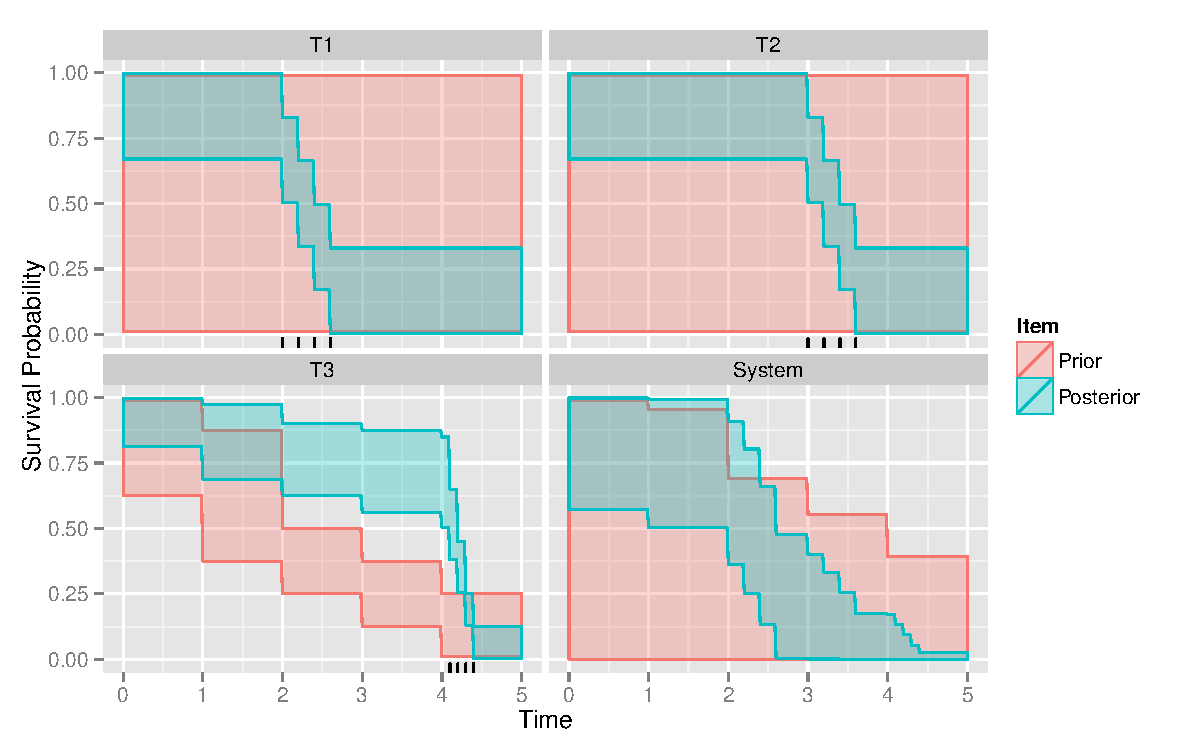
\includegraphics[width=\textwidth]{3comp-latefailures}\\
{\small \qquad(joint work with Louis Aslett and Frank Coolen)}
\end{frame}

\frame{\frametitle{Example: Scaled Normal Data}
\begin{tikzpicture}
\uncover<1>{%
\node (0,0) {\begin{minipage}{0.99\textwidth}%
\begin{block}{Example: Scaled Normal Data}
\begin{tabular}{r|lcl}
Data :           & $\x\mid\mu$        & $\sim$ & $\norm(\mu,1)$\\[0.5ex] %\sigma_0^2)$ \quad ($\sigma_0^2$ known)\\[0.5ex]
conjugate prior: & $\mu\mid\nzg,\yzr$ & $\sim$ & $\norm(\yzr, 1/\nzg)$  \\[0.5ex]
\cline{1-4}
posterior:       & $\mu\mid\nng,\ynr$ & $\sim$ & $\norm(\ynr, 1/\nng)$ \quad ($\tau(\x)/n = \bar{x}$)\rule{0ex}{2.5ex} %& \\[0.5ex]
\end{tabular}
\end{block}\vspace*{18ex}\end{minipage}};}
\uncover<2>{%
\node (0,0) {%
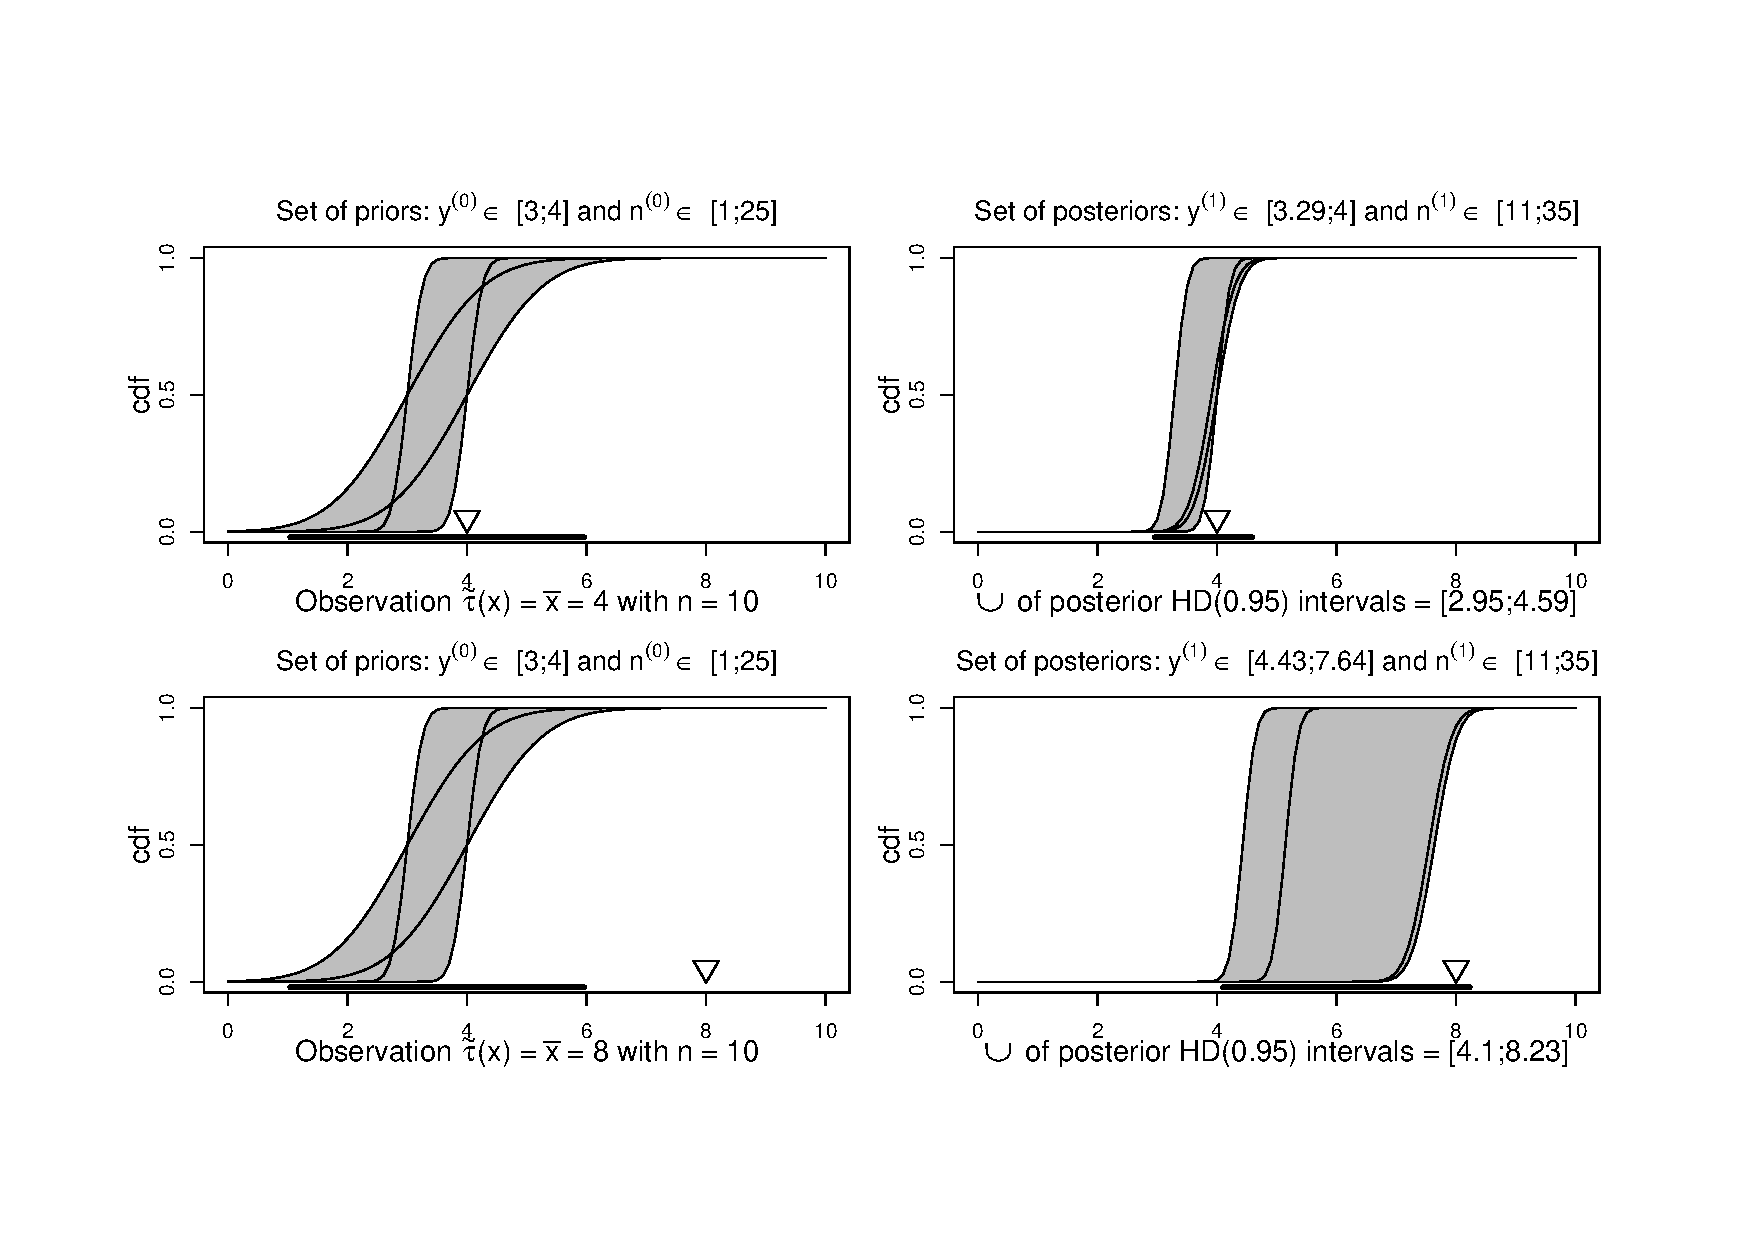
\includegraphics[trim = 20mm 20mm 20mm 25mm, clip, width=\textwidth]{jstp-paper_nv_nvar_vertfu01_081128}};}
\end{tikzpicture}
}

\begin{frame}[label=othermodels-back]{General Model Properties}
\uncover<1->{%
Good inference properties \hyperlink{othermodels-app}{\small (cf.\ other models based on sets of priors)}}
\begin{itemize}%[<+->]
%\note<10>[item]{In contrast to other models based on sets of priors,\\
%this model is easy to handle and to elicit,\\ and has very favourable inference properties}
\item<1-> $n \to \infty$\hspace*{1.6ex}%
%\uncover<2->{\then\ \ $\ynr$ values in $\PNc \to \frac{\tau(\x)}{n}$\hspace*{0.9ex}}%
%\uncover<3->{\then\ \ `Bayesian consistency'}
\uncover<2->{\play\ $\ynr$ stretch in $\PNc \to 0$\hspace*{1.6ex}}%
\uncover<3->{\play\ precise inferences}
\item<4-> larger $\nzg$\hspace*{1.6 ex}\play\ larger $\PNc$ \hspace*{8.84ex}\play\ more vague inferences
%\note<10>[item]{larger $\nzg$ as compared to $n$:
%more weight on imprecise prior $\MZ$\\ leads to more imprecise posterior $\MN$}
\item<5-> larger range of $\yzr$ in $\PZc$\hspace*{1.6ex}\play\ larger range of $\ynr$ in $\PNc$\\[0.5ex]
\hspace*{30.02ex}\play\ more vague inferences
%\note<10>[item]{more imprecise prior $\MZ$ leads to more imprecise $\MN$}
\end{itemize}
\uncover<6->{%
Model very easy to handle:}
\begin{itemize}%[<+->]
\item<6-> Hyperparameter set $\PZc$ defines set of priors $\MZ$
\item<7-> Hyperparameter set $\PNc$ defines set of posteriors $\MN$
\item<8-> $\PZc \to \PNc$ is easy: $\nng = \nzg + n$, $\ynr = \frac{\nzg}{\nzg + n}\,\yzr + \frac{n}{\nzg + n}\cdot\frac{\tau(\x)}{n}$
%\item<9-> For quantities linear in posteriors, bounds are attained at ``pure'' posteriors $p(\psib\mid\nng,\ynr)$
%\then\ optimise over $\PNc$ (not over $\MN$)
\item<9-> Often, optimising over $(\nng,\ynr) \in \PNc$ is also easy:\\
\alert{closed form solution} for $\ynr$ = posterior `guess' for $\frac{\tau(\x)}{n}$ (think: $\bar{x}$)\\
when $\PZc$ has `nice' shape
\end{itemize}
\end{frame}

\frame{\frametitle{Hyperparameter Set Shapes}
%graphs line, rectangle, eggplant
\vspace*{-4ex}
\begin{tikzpicture}
%\uncover<1>{\node {\includegraphics[scale=0.75]{../R/shape0.pdf}};
%            \draw[-stealth,very thick] (-1,-0.4) -- (2.3,1.1) node [above,midway,sloped] {+ data};}
\uncover<1>{\node {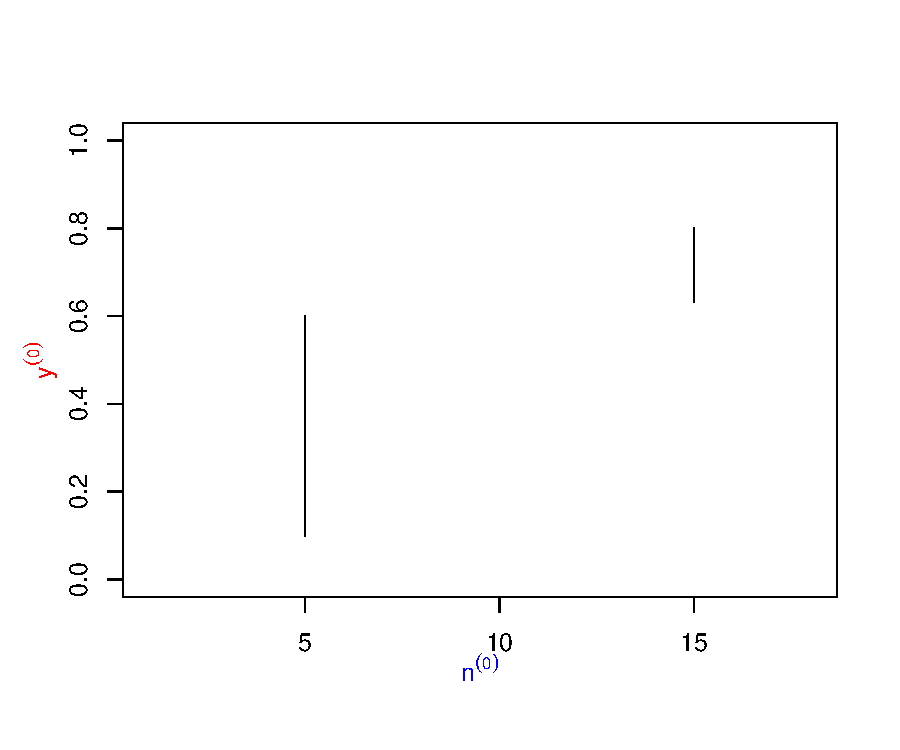
\includegraphics[scale=0.75]{shape1}};
            \draw[-stealth,very thick] (-1,-0.4) -- (2.3,1.1) node [above,midway,sloped] {+ data};}
\uncover<2>{\node {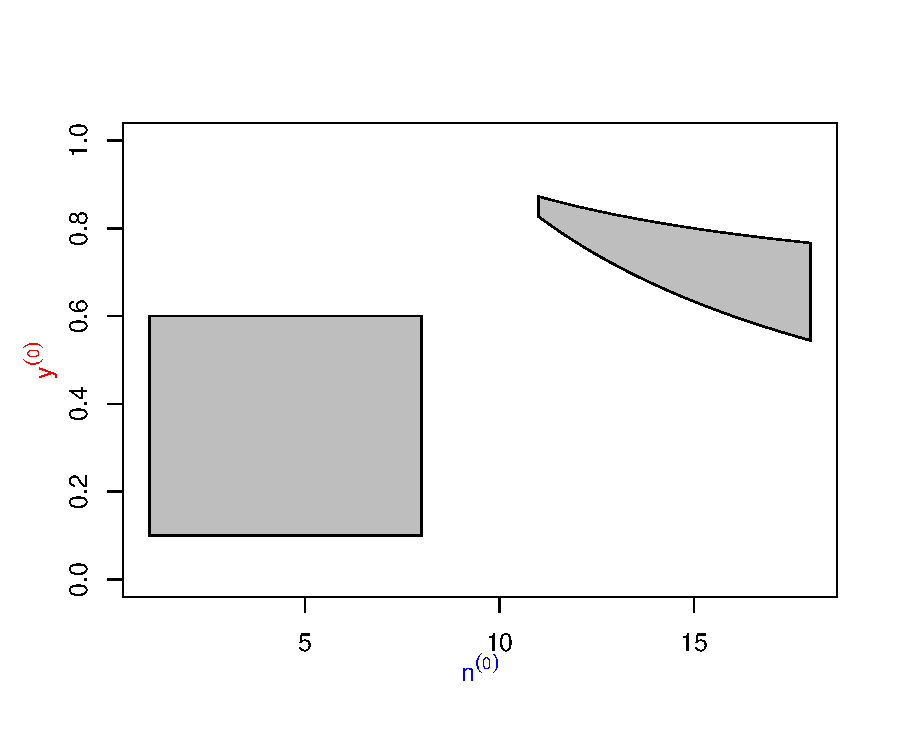
\includegraphics[scale=0.75]{shape2}};
            \draw[-stealth,very thick] ( 0,-0.5) -- (2.3,1.1) node [above,midway,sloped] {+ data};}
\uncover<3>{\node {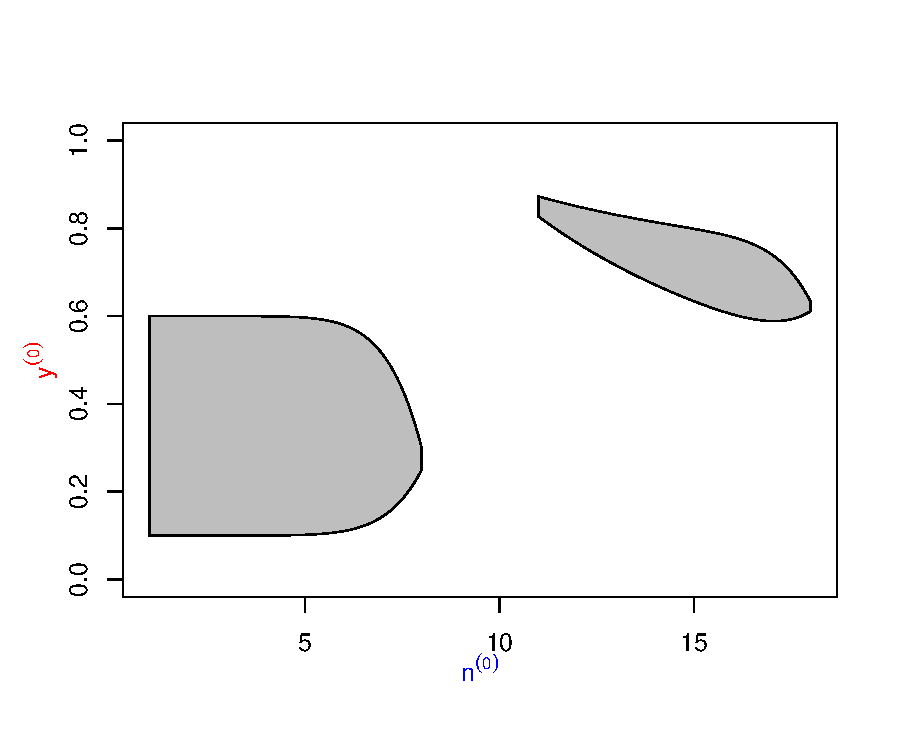
\includegraphics[scale=0.75]{shape3}};
            \draw[-stealth,very thick] ( 0,-0.5) -- (2.3,1.1) node [above,midway,sloped] {+ data};}
\end{tikzpicture}
}

\begin{frame}[label=luck-back]{Hyperparameter Set Shapes}
\begin{itemize}%[<+->]
\item<1-> Set shape is crucial modeling choice:\\ %A range of $\nzg$ values is needed for \pdc\ reaction
trade-off between model complexity and model behaviour
% \begin{itemize}
\item<2-> $\PZc\! = \nzg \times [\yzlr, \yzur]$
 %{\small (Walley\,1996;\,Quaghebeur\,\&\,de\,Cooman\,2005)}:\\
 {\footnotesize \parencite{1996:walley::idm,2005:quaeghebeurcooman}:}\\
 $\PNc\! = \nng \times [\ynlr, \ynur]$ \play\ optimise over $[\ynlr, \ynur]$ only,\\
 \hspace*{20.9ex}but no prior-data conflict sensitivity
\item<3-> $\PZc\! = [\nzlg,\nzug] \times [\yzlr, \yzur]$ %{\small (Walley 1991; Walter \& Augustin 2009)}:\\
 {\footnotesize \parencite{1991:walley,2009:WalterAugustin}:}\\
 $\PNc$ have non-trivial forms (banana / spotlight), but prior-data conflict sensitivity and closed form for $\min / \max \ynr$ over $\PNc$.\\
 For other inferences, \textbf{R} package \hyperlink{luck-app}{\texttt{luck}} implements optimisation
 over $\PNc$ via box-constraint optimisation over $\PZc$
% \end{itemize}
\item<4-> Other set shapes possible, but may be more difficult to handle %elicit
%\item<8-> Prior information may be such that range of $\yzr$ changes with $\nzg$ (or vice versa)
\end{itemize}
\end{frame}

\begin{frame}[label=boat-back]{Hyperparameter Set Shapes}
%\hspace*{-2ex}%
%\uncover<2->{%
%\vspace*{-7ex}%
%\begin{center} %trim=l b r t
\vspace*{2ex}%
Parameter set shape for strong prior-data agreement {\small \parencite[A.2]{2013:diss-gw}}
\hyperlink{boat-app}{%
\begin{tikzpicture}
%\includegraphics[trim = 40mm 35mm 40mm 45mm, clip, width=\textwidth]{../R/boatshape-durham0913} % width=8, height=6
\uncover<1>{\node {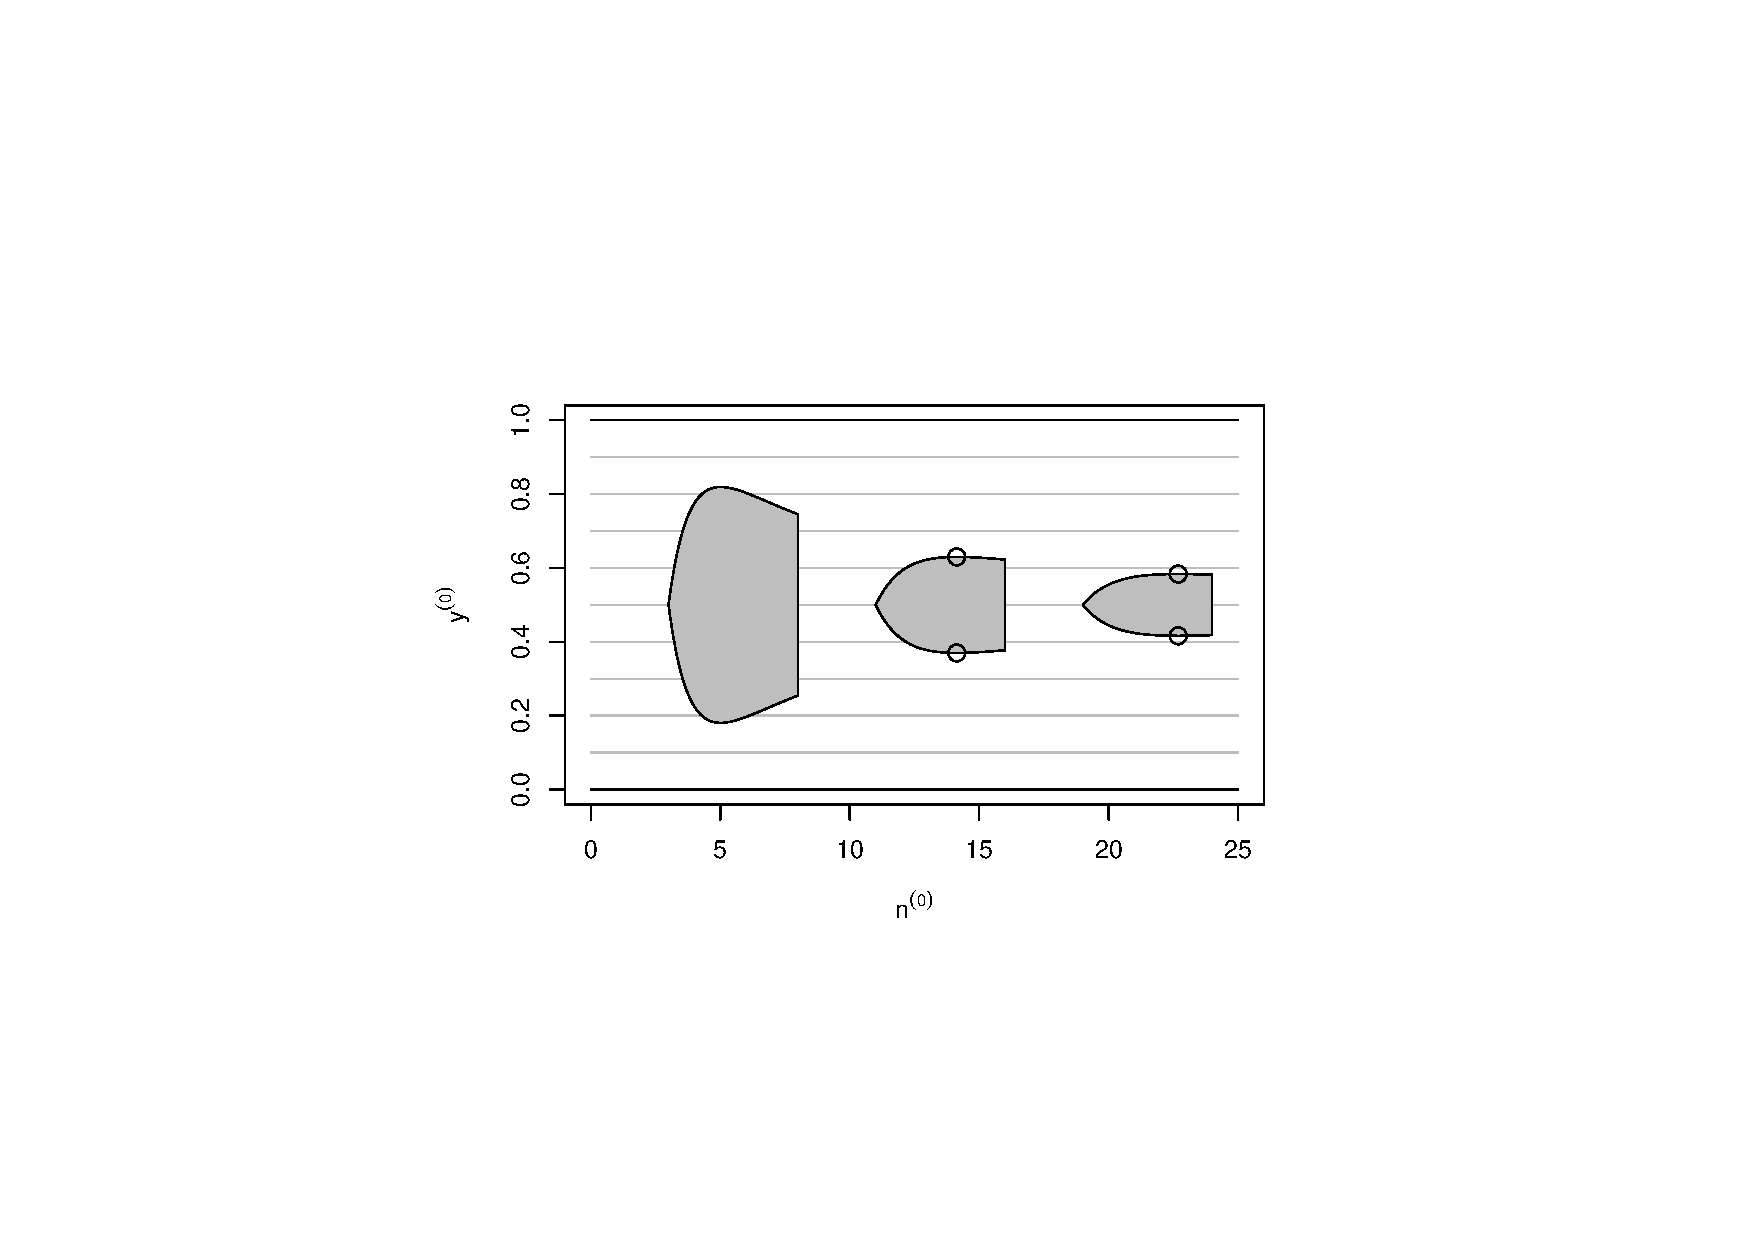
\includegraphics[trim = 70mm 52.5mm 70mm 65mm, clip, width=\textwidth]{boatshape-defense-1}};} % width=6, height=4.5
\uncover<2>{\node {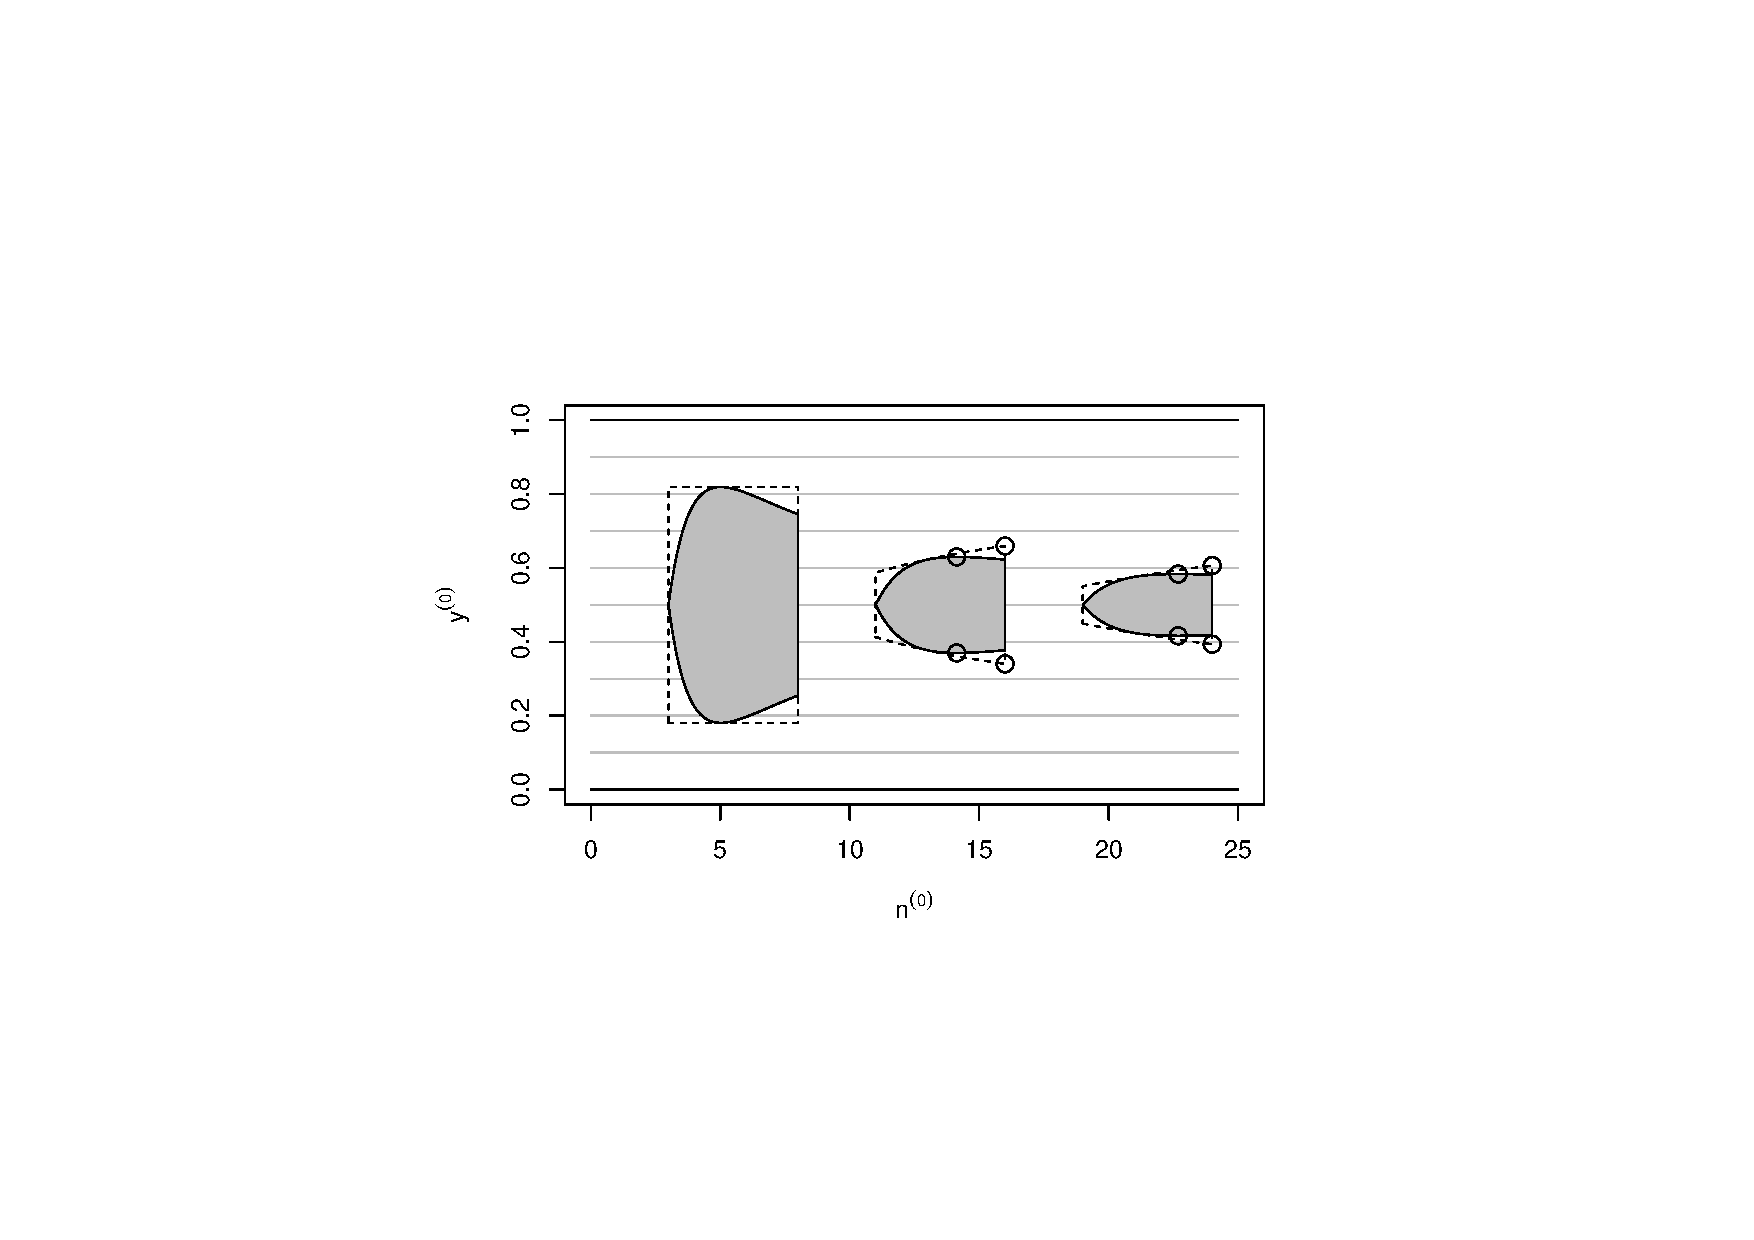
\includegraphics[trim = 70mm 52.5mm 70mm 65mm, clip, width=\textwidth]{boatshape-defense-2}};} % width=6, height=4.5
\end{tikzpicture}
}%
%\end{center}%}
\end{frame}

\begin{frame}[label=luck-back-summary]{Summary}
\begin{itemize}%[<+->]
\item<1-> Conjugate priors are a convenient tool for Bayesian inference\\ but there are some pitfalls
 \begin{itemize}%[<+->]
 \item Hyperparameters $\nzg,\yzr$ are easy to interpret and elicit
 \item Averaging property makes calculations simple, but leads to
 inadequate model behaviour in case of prior-data conflict
 \end{itemize}
\item<2-> Sets of conjugate priors maintain advantages \& mitigate issues %find a sweet spot in between
 \begin{itemize}%[<+->]
 \item Sets of posteriors adequately reflect vague prior information,\\ the amount of data, and prior-data conflict %uncertainties from
 \item Hyperparameter set shape is important %a crucial modeling choice
 \item Reasonable choice: \emph{rectangular} $\PZc = [\nzlg, \nzug] \times [\yzlr, \yzur]$:\\
 \emph{``generalised iLUCK-models''} {\footnotesize\parencite{2009:WalterAugustin,2013:diss-gw}},\\
 \textbf{R} package \hyperlink{luck-app}{\texttt{luck}} {\footnotesize\parencite{luck-package}}
 %(Walter \& Augustin 2009: \emph{generalised iLUCK-models}, \hyperlink{luck-app}{\texttt{luck}})
 \item Bounds for prior hyperparameters $(\nzg,\yzr)$\\ are easy to interpret and elicit
 \item Additional imprecison in case of prior-data conflict\\
 leads to \alert{cautious inferences if, and only if, caution is needed}
 %\item Shape for more precision in case of strong prior-data agreement is in development
 %(joint work with Frank Coolen and Mi\c{k} Bickis)
 \end{itemize}
\end{itemize}
\end{frame}

\begin{frame}[allowframebreaks]{References}
%\begin{frame}[allowframebreaks]{References}
%
%  \bibliographystyle{plain}
%  {\scriptsize
%  \bibliography{../_diss/v1/bib/other-refs,../_diss/v1/bib/itip-refs} 
%  }
\printbibliography[heading=none]
\end{frame}


%---- bonus material


\begin{frame}[label=othermodels-app]{Other models using sets of priors
\hyperlink{othermodels-back<3>}{\beamerreturnbutton{top}} \hyperlink{othermodels-back<10>}{\beamerreturnbutton{bottom}}}
\begin{itemize}
\item Neighbourhood models
\begin{itemize}
\item set of distributions `close to' a central distribution $P_0$
\item common in robust Bayesian approaches 
\item example: $\varepsilon$-contamination class:
$\{ P : P = (1-\varepsilon) P_0 + \varepsilon Q, Q \in \mathcal{Q} \}$
\item not necessarily closed under Bayesian updating
\end{itemize}
\item Density ratio class / interval of measures 
\begin{itemize}
\item set of distributions by bounds for the density function $f(\vartheta)$:
\begin{align*}
\mathcal{M}_{l,u} = \big\{ f(\theta) :
\exists c \in \posreals: l(\theta) \le c f(\theta) \le u(\theta)\big\}
\end{align*}
\item posterior set is bounded by updated $l(\theta)$ and $u(\theta)$
\item $u(\theta)/l(\theta)$ is constant under updating\\
\quad\play\ size of the set does not decrease with $n$\\
\quad\play\ too vague posterior inferences
\end{itemize}
\end{itemize}
\end{frame}

\begin{frame}[label=luck-app]{\textbf{R} package \texttt{luck} %
\hyperlink{luck-back<4>}{\beamerreturnbutton{set shapes}} %
\hyperlink{luck-back-summary<2>}{\beamerreturnbutton{summary}}}
\begin{itemize}
\item \texttt{S4} implementation of the general canonical prior parameter structure
with rectangular sets $\PZc = [\nzlg, \nzug] \times [\yzlr, \yzur]$
\item lean subclasses for concrete sample distributions\\
(currently implemented: scaled normal, exponential)
\item available on R-Forge:\\[1.5ex]
{\footnotesize \url{install.packages("luck", repos="http://R-Forge.R-project.org")}\\[1.2ex]
or\\[1.2ex]
\url{install.packages("http://download.r-forge.r-project.org/src/contrib/luck_0.9.tar.gz", repos = NULL, type = "source")}}
%{\small (issue: \texttt{S4} classes and \texttt{S3}-style documentation seem to be incompatible)} 
\end{itemize}
\end{frame}
\addtocounter{framenumber}{-1} 

\begin{frame}{\textbf{R} package \texttt{luck} %
\hyperlink{luck-back<4>}{\beamerreturnbutton{set shapes}} %
\hyperlink{luck-back-summary<2>}{\beamerreturnbutton{summary}}}
\vspace*{-5ex}
\hspace*{10ex}
\begin{tikzpicture}[class/.style={draw, rectangle split, rectangle split parts=3, %
                                  every text node part/.style={text centered}, %
                                  font=\ttfamily, %
                                  fill=gray!30, text width=45mm, thick}, %
                    point/.style={coordinate},
                    transform canvas={scale=0.8}]%every node/.style=draw]
\node [class] (luck) at (0,0) {LuckModel \nodepart{second} \gruen{n0}: matrix \\
                                         \rot{y0}: matrix \\
                                         data: LuckModelData
                                         \nodepart{third}
                                         show() \\
                                         plot() \\
                                         unionHdi() \\
                                         \quad \vdots};
\node [coordinate, below=0.4cm of luck] (p0) {};
\node [coordinate, left=0.4cm of p0] (p1) {};
\node [class, text width = 47mm] (scalednormal) [below=0.4cm of p1] {ScaledNormalLuckModel\phantom{p} %
                                                                        \nodepart{second} \phantom{pS}
                                                                        \nodepart{third} singleHdi()\phantom{p}\\};
\draw [stealth'-, thick] (luck.south) -- (p0) -- (p1) -- (scalednormal.north); %node [midway,right,draw=none] {inherits};
\node[class, text width=45mm] (poisson) [right=0.5cm of scalednormal] {ExponentialLuckModel %
                                                                        \nodepart{second} \phantom{pS}
                                                                        \nodepart{third} singleHdi()\phantom{p}\\};
\node[class, text width=35mm, double copy shadow={shadow xshift=1mm,shadow yshift=-1mm}] %
 (more) [right=0.5cm of poisson] {\phantom{pS}\ldots\phantom{pS} \nodepart{second} \phantom{pS}
                                                                 \nodepart{third} singleHdi()\phantom{pS}\\};
\node [coordinate, above=0.4cm of poisson] (p2) {};
\draw [thick] (p0) -- (p2) -- (poisson.north);
\node [coordinate, above=0.4cm of more] (p3) {};
\draw [thick] (p2) -- (p3) -- (more.north);
%\draw[->] (0,0) -- (1,0);
\begin{scope}[transform canvas={scale=0.75}]
%\draw[->] (0,0.5) -- (1,0.5);
%\node [coordinate] (lmd) [right=0.5cm of luck] {}; 
\node [class] (data) at (6.8,1.5) {LuckModelData \nodepart{second} tauN: matrix\\ rawData: matrix
                                                             \nodepart{third} show()};
\node [coordinate, below=0.4cm of data] (dp0) {};
\node [coordinate, left=0.4cm of dp0] (dp1) {};
\node[class, text width=37mm] (scalednormaldata) [below=0.4cm of dp1] {ScaledNormalData\phantom{p} \nodepart{second} \phantom{h}
                                                                                                   \nodepart{third} show()};
\node[class, text width=37mm] (poissondata) [right=0.5cm of scalednormaldata] {ExponentialData \nodepart{second} \phantom{h}
                                                                                               \nodepart{third} show()};
\node[class, text width=30mm, double copy shadow={shadow xshift=1mm,shadow yshift=-1mm}] %
 (moredata) [right=0.5cm of poissondata] {\phantom{pD}\ldots\phantom{pD} \nodepart{second} \phantom{h}
                                                                         \nodepart{third}  show()};
\draw [stealth'-, thick] (data.south) -- (dp0) -- (dp1) -- (scalednormaldata.north); %node [midway,right,draw=none] {inherits};
\node [coordinate, above=0.4cm of poissondata] (dp2) {};
\draw [thick] (dp0) -- (dp2) -- (poissondata.north);
\node [coordinate, above=0.4cm of moredata] (dp3) {};
\draw [thick] (dp2) -- (dp3) -- (moredata.north);
\end{scope}
\node [coordinate] (snake) at (2.75,1.025) {};
\draw [dashed, very thick, -stealth'] (2.5,0.35) .. controls +(right:4mm) and +(up:4mm)
                                      .. (snake) .. controls +(up:4mm) and +(left:8mm) .. (3.2,1.7);
\end{tikzpicture}
\end{frame}

\begin{frame}[label=boat-app]{Strong Prior-Data Agreement Modelling \hyperlink{boat-back<2>}{\beamerreturnbutton{}}}
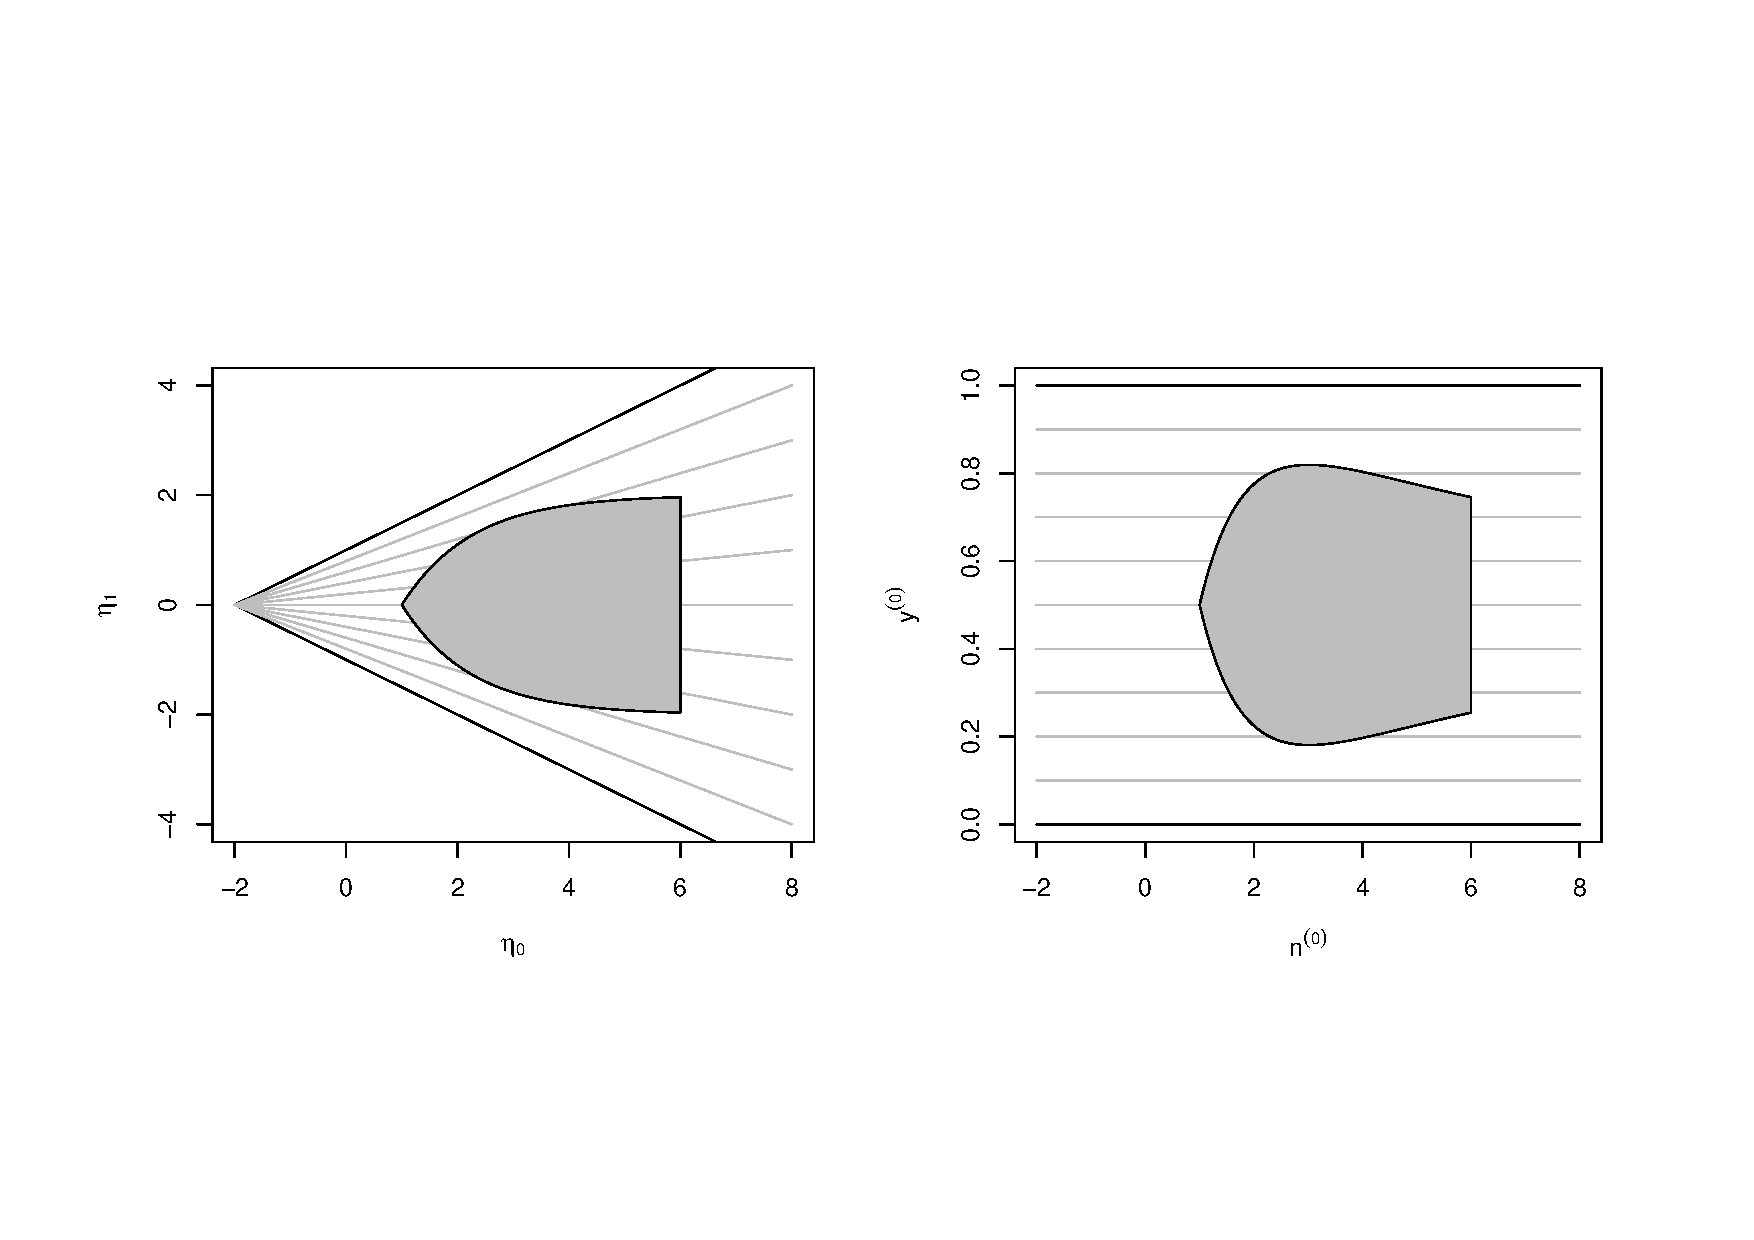
\includegraphics[trim = 15mm 45mm 25mm 60mm, clip, width=\textwidth]{boatshape-prior}
\end{frame}

%---- reset total frame number
\addtocounter{framenumber}{-3} 

\end{document}

\begin{block}{Beta-Binomial Model}
\begin{tabular}{r|lcl}
data :           & $s \mid p$          & $\sim$ & $\bin(n,p)$   \\[0.5ex]
conjugate prior: & $p \mid \nzg, \yzr$ & $\sim$ & $\be(\nzg,\, \yzr)$  \\[0.5ex]
\cline{1-4}
posterior:       & $p \mid \nng, \ynr$ & $\sim$ & $\be(\nng,\, \ynr)$\rule{0ex}{2.5ex}
%\quad ($\frac{\tau(\x)}{n} = \frac{s}{n}$)\rule{0ex}{2.5ex}
\end{tabular}
\end{block}

